\begin{flushleft}
    \section{Analysis}
        \subsection{Statement of Investigation}
            \large
            \vspace{0.2cm}
            I plan to investigate Machine Learning and Neural Networks by developing a Survival Simulation environment 
            in which a character will be controlled by a Machine Learning algorithm. \\
            \vspace{0.2cm}
            The Machine Learning Algorithm I choose to implement will most likely require lots of Complex Maths, from prior knowledge
            I know that Matrices and Calculus are heavily used within Neural Networks. Most of the Maths I will have 
            covered in my Maths and Further Maths Lessons, but some will require independent research on my Part. \\
            \vspace{0.2cm}
            The survival simulation will be Procedurally Generated and present multiple challenges 
            towards this character in order to provide a complex problem for it to solve. The procedural generation will
            be based upon a seed, and will generate Terrain which the character has to explore and navigate. The challenges 
            could be things like collecting items, or having to avoid/kill enemies which are actively tracking the character 
            and trying to hinder its progress. \\
            \vspace{0.2cm}
            The key question I aim to answer with this investigation is:

            \begin{center}
                \vspace{0.3cm}
                \textbf{Can I develop a Machine Learning Algorithm to survive in a pseudorandom, open-world environment?}
                \vspace{0.3cm}
            \end{center}

            Whether I have answered this question or not should be clear. I will be able to specifically measure the Algorithm's ability 
            to survive by observing its actions in given situation. If the Algorithm directs the character into danger
            on a regular basis, it clearly isn't achieving this goal. If the Algorithm doesnt outright solve the given simulation, 
            I will have to determine to what extent it manages the to solve the simulation. \\
            \vspace{0.2cm}
            I can determine this by asking more specific questions, proposed below: \\

            \begin{enumerate}
                \item \textbf{Does the Algorithm draw links between specific elements and danger?}
                \item \textbf{How well does the Algorithm perform with specific tasks?}
                \item \textbf{If the problem is altered to be simpler does the Algorithm perform better?}
                \item \textbf{Can I fine tune the Algorithms Parameters to get better results?}
            \end{enumerate}

            These more specific questions will allow me to determine to what extent the Algorithm can solve the problem.
            I hope to dive more in depth into answering these in my Evaluation Section later in the project. \\
            \vspace{0.2cm}
            The First Question I feel is important because it shows a reasonably high level of understanding of the problem
            if it can somehow make links between specific parts of its input and determine that they are in fact dangerous. \\
            \vspace{0.2cm}
            The Second Question may be harder to answer, because I will have to somehow determine just how well it 
            performs doing something like Collecting Items, or Killing Enemies. This can't really be analysed through
            pure numbers and instead would have to determined through surveying the Algorithm as it works. \\
            \vspace{0.2cm}
            The Third Question will definitely be something to test for, I think it will be relatively easy to tell if
            adjusting the problem shows a noticeable improvement/deterioration in ability to solve the Simulation. \\
            \vspace{0.2cm}
            The Fourth Question should be something quite easy to determine if it makes an impact, but overall shall
            be needed when trying to find the optimal setup for the Algorithm such that it performs its best. \\
        \subsection{Background}
            \vspace{0.2cm}
            Machine Learning is an ever evolving field with Limitless Potential. The key concept behind it is built around training
            Mathematical Models to recognize patterns within the Input Data. Any error found within the output of the the Model is then
            taken into account, causing updates to Weights and Biases, eventually forming an optimal Model/Policy. These Mathematical 
            Models vary in complexity massively, from simple Equations to complex interlinking layers of Nodes. Applications of such 
            algorithms range from finding Linear Regression Lines, to Automating Complex Multi-Step Tasks. Commonly used within Machine 
            Learning is the concept of a Neural Network. It's formed from a series of layers which hold Weights and Biases between the 
            previous and subsequent layer. To my current understanding they utilise Matrix Operations to speed this process up. \\
            \vspace{0.2cm}
            I find this concept quite interesting, and have wanted to try gain a deeper understanding into the different 
            algorithms behind Machine Learning for a while now. This is the basis of my Investigation and Project. By the end
            of completing this Investigation I will hopefully be able to fully explain the process behind the Algorithm I choose
            to implement. \\
            \vspace{0.2cm}
            Procedural Generation is also an interesting topic. It's revolves around utilising an Algorithm to generate values. In my 
            case I will be using these values for Terrain Generation. Algorithms like this are often seeded, meaning they will generate 
            deterministically with the same values if the same seed is used. Procedural Generation could also be used for Loot Systems
            in Video Games, or generating VFX for Films. This is a less important part of my investigation though, due to being
            the secondary aspect.
            \vspace{0.2cm}
        \subsection{Expert}
            \vspace{0.2cm}
            For my expert I approached one of my friends, Shaun, who has prior experience with Machine Learning. He has
            created his own Handwritten Digit Recognition Network before, along with using Python Libraries such as 
            \textit{PyTorch} to train an agent to play the game \textit{Flappy Bird}, among other ML projects. He has 
            a much better understanding of Machine Learning than me currently, so hopefully he will be a good resource 
            as I develop my project. \\
            \vspace{0.2cm}    
            I chose Shaun as my Expert because of his prior experience with Machine Learning, but also because he showed interest
            in the final results of my Investigation. He found the idea of trying to generalise a Machine Learning Algorithm
            to function effectively within a Procedurally Generated Environment intriguing. He commented to me outside of the
            two Interviews I conducted with him, that he's \textit{"Interested in the final results of the Program"}. He also
            mentioned the Idea of comparing multiple Algorithms against eachother, but I felt like this would be an unreasonable
            task for an NEA Project. \\
            \vspace{0.2cm}    
        \subsection{Initial Research}
            \subsubsection{First Interview}
                \large
                As part of my Investigation I approached my friend Shaun, who has Experience with Machine Learning.
                I formed a list of questions to ask him, the responses are paraphrased for clarity. I mainly wanted to gain an idea of 
                what Machine Learning algorithm would suit my project the best. So I targetted my questions towards this. \\
                \vspace{0.2cm}
                \begin{enumerate}
                    \item {\large What are your first impressions of my project?} \\
                    \vspace{0.2cm}
                    “Your project is definitely very complex and if finished will tick a lot of the boxes needed for Full Marks. There are lots
                    of layers of complexity along with room for good Object Orientated Design. I find your project quite intriguing and would be
                    interested to see how your well your final implemented Machine Learning Algorithm fares in a Procedurally Generated Environment.”

                    \item {\large What Machine Learning Algorithms do you think would be relevant to my project?} \\
                    \vspace{0.2cm}
                    "Without pushing your complexity too far I think you should look into Deep Q Learning, I believe it has the
                    possibility of solving your problem if not too complex. Because of that you may way want to keep your simulation as minimal
                    as possible in order to give your Agent a chance. If you wanted to go further you could implement a Convolutional Neural Network, 
                    but this will add to the Complexity and take more time to program."

                    \item {\large Would User Defined Parameters be helpful?} \\
                    \vspace{0.2cm}
                    "The ability to dynamically change the parameters through a JSON file or similar would be very useful. Especially to users who
                    have little to no experience with it beforehand. The ability to change things like the Procedural Generation, Enemy Counts, 
                    Network Structure etc would be the perfect addition to your project."

                    \item {\large What Procedural Generation method would be best for my Project?} \\
                    \vspace{0.2cm}
                    "I only have experience with Perlin Noise, but I think that it would be a great fit for your Project. It uses simple vector Maths
                    to calculate Gradient Noise, and is relatively simple to understand and Program. There are other Procedural Generation Methods
                    I'm aware of like Diamond Square or Simplex Noise, but both of those are much more complicated to my understanding."

                    \item {\large How complex should I make my Simulation?} \\
                    \vspace{0.2cm}
                    "I would stick to a relatively simple simulation at first, and then if your agent is successful at solving it, you can add more
                    to test the limits of your network after. Dynamic threats like Enemies which follow the Agent which it can attack would provide a base 
                    complex problem to start off with. Other problems could be collecting items or a simple Food Collection system with a Hunger Meter."

                    \item {\large How should I determine if my project is successful?} \\
                    \vspace{0.2cm}
                    "You could log a graph of Loss compared to Time, and in theory if your agent is learning it will successfully reduce the average Loss 
                    the more training it receives. You could use this graphed data as supporting evidence when evaluating your project. You could probably
                    save data and plot it using a Graphing Library of some sort, there's bound to be one with your language of choice."

                    \item {\large What should I focus my Initial Research on?} \\
                    \vspace{0.2cm}
                    "It would be beneficial to you to research the Maths behind Neural Networks, specifically for Forward Propagation
                    and Back Propagation. The Maths behind it can get very complicated, along with being very hard to debug if a small error is made.
                    They both heavily rely on Matrix Operations, so if you're not familiar with those you should get up to speed."
                \end{enumerate}
            \subsubsection{Evaluation of First Interview}
                My Experts input as part of my Initial Research is useful because it gives me a better understanding of the areas I should target my
                research on. Below is my thoughts on various parts of the Interview:

                \begin{itemize}
                    \item I will definitely focus alot of my research on Neural Networks and Deep Q Learning. Though I will look into other
                    alternatives which I could use.

                    \item User Defined Parameters will definitely be included in the design of my project. I feel as though this would be
                    very helpful for testing, being able to find tune needed Parameters without having to chance them in the code would be useful.

                    \item Perlin Noise sounds like a good method of generating Terrain. I will include this as part of my Research into Algorithm 
                    I might utilise.

                    \item This guide for the complexity of my simulation will be useful when designing it. I also like his idea regarding collecting food to 
                    stay alive with a hunger bar. Implementing more complex problems like this could be difficult for the Algorithm to solve though. 
                    
                    \item Graphing the Average Loss using a Graphing Library would be helpful and support the Evaluation of my Project. It would mean
                    that I'd need to include a Data Logger as part of the design of my project, as well as a library which can plot this Data.

                    \item Pointing me towards learning the complexities behind Forward and Back Propagation is definitely a good starting point
                    as part of my initial research. He also pointed me towards a few helpful resources for learning these two concepts. I will definitely
                    read through these.
                \end{itemize}
            \subsubsection{Existing Investigations} 
                \paragraph{Crafter} \mbox{} \\
                    \vspace{0.2cm}
                        In my research on the Internet I discovered a project called \textit{Crafter}. \\

                        \vspace{0.2cm}
                        \centerline{\textit{https://github.com/danijar/crafter}}
                        \vspace{0.2cm}

                        Crafter is described to be \textit{"Benchmarking the Spectrum of Agent Capabilities"}, and is utilised
                        in conjunction with Machine Learning Algorithms such as \textit{DreamerV2}, \textit{PPO} and \textit{Rainbow}. Crafter poses significant
                        challenge towards its Player, requiring high levels of generalization, long-term reasoning, and complex 
                        problem-solving. If the Machine Learning algorithm in question fails to achieve one of these aspects it will 
                        struggle to full "Solve" the simulation. \\

                        \vspace{0.2cm}

                        High levels of generalization are required when training a Machine Learning algorithm, if this is not achieved then
                        your network will only lend itself to a single Dataset/Problem. An example of this would be training a network used
                        to recognize handwritten digits on only one way of writing 4's, if presented with an input for a different type of 
                        4 it may not recognize it and identify it incorrectly. \\
                        
                        \vspace{0.2cm}

                        Long-Term reasoning is a complex problem to solve in the context of Machine Learning, current Machine Learning models
                        struggle to deal with this problem. This is dealt with by using algorithms built to mimic "memory". A common 
                        implementation of this is Experience Replay which stores states in a queue, and relearns from it after every N ammount
                        of steps. \\

                        \vspace{0.2cm}

                        A complex reward and action system may take time for an algorithm to learn, but it certainly is possible with current
                        Machine Learning Models. Crafter utilizes a complex action system with a flow chart determining which Action can be taken
                        given the current state of the simulation. Below is shown the Complex Flow Chart of Actions: \\

                        \vspace{0.2cm}
                        \begin{center}
                            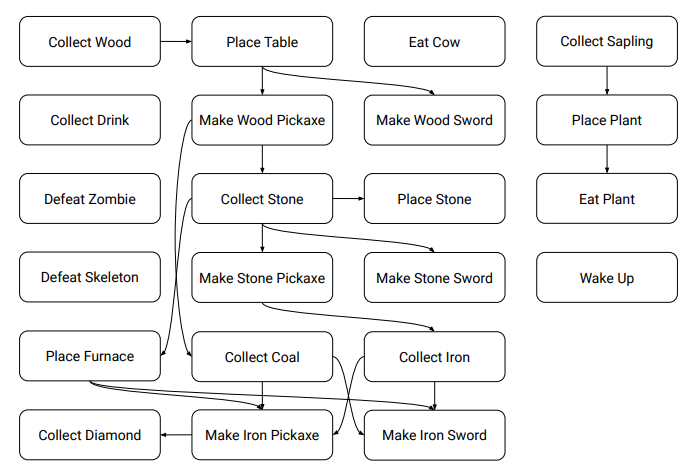
\includegraphics[width=12cm]{Images/InitialResearch/CrafterComplexActionSystem.PNG} \\
                            Complex action system as shown in the Paper "Benchmarking the Spectrum of Agent Capabilities" \\
                        \end{center}
                        \vspace{0.2cm}

                        Crafter manages to achieve quite high success rates with various Algorithms, but they still fail to overcome, or even match
                        human standards. This is likely due to the complexity of the problem, and in theory will be solvable within the near future
                        as Machine Learning advances over the next few years. This is why I plan to create a simpler simulation which the Agent will
                        be more likely to be able to solve. Below is shown the Success Rate Data for both Algorithms and Human Experts. \\

                        \begin{figure}[H]
                            \centering
                            \subfloat[\centering Success Rate of Algorithms]{{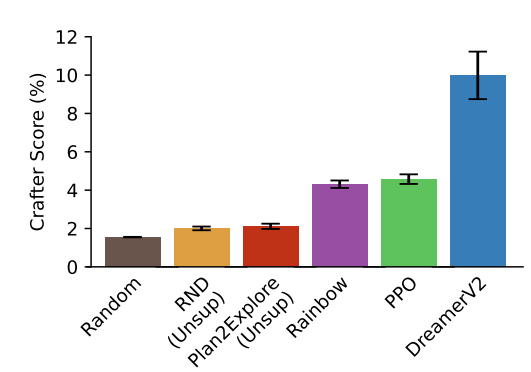
\includegraphics[width=7cm]{Images/InitialResearch/CrafterMLTrainingData.PNG}}}
                            \qquad
                            \subfloat[\centering Comparison Against Human Data]{{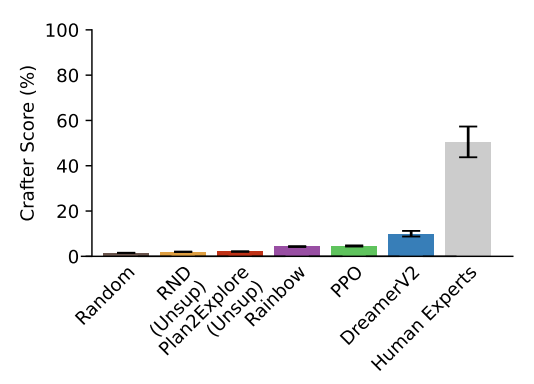
\includegraphics[width=7cm]{Images/InitialResearch/CrafterMLTrainingData+Human.PNG}}}
                            \caption*{Data from "Benchmarking the Spectrum of Agent Capabilities"}
                        \end{figure}

                        While I would love to create a simulation similar to crafter, it is very complex and would take a long time to develop. Yet
                        would not net many marks in the process. Overall I feel like Crafter is a good example that my project is possible, but will
                        require a complex Machine Learning Model in order to achieve reliable results from my Investigation.

                \paragraph{Minecraft} \mbox{} \\
                    \vspace{0.2cm}
                    Minecraft is a \textit{very} popular Game. It's a sandbox game, meaning that the player can do almost anything they want.
                    The game is formed from blocks which can be broken or placed, along with a plethora of items, enemies, passive animals
                    and more. It has infinite terrain generation, and explicitly uses Perlin Noise. The seed of the noise determines
                    all the terrain generation, loot tables, random structures, caves, etc. \\
                    
                    \vspace{0.2cm}

                    First it starts off on a very broad level, painting a basic topographical map of the world. It uses Perlin Noise to sample
                    a height value for each chunk, where chunks are 16x16 areas of blocks. Then within these chunks the game uses the Diamond Square
                    algorithm to interpolate between it and the surrounding chunks, creating blocks where the terrain should be. This produces an 
                    entirely deterministic results based upon the seed.\\

                    \vspace{0.2cm}

                    Secondly, the Caves are generated using Perlin Worms, which travel in deterministic directions based on their starting position.
                    These worms dig through the terrain carving out caves which can then be traversed by the player. Within these Caves spawn water
                    sources, pools of lava, useful ores. All of these are deterministically generated by the original seed. \\ 


                    \begin{figure}[H]
                        \centering
                        \subfloat[\centering Example of Minecraft's Terrain Generation]{{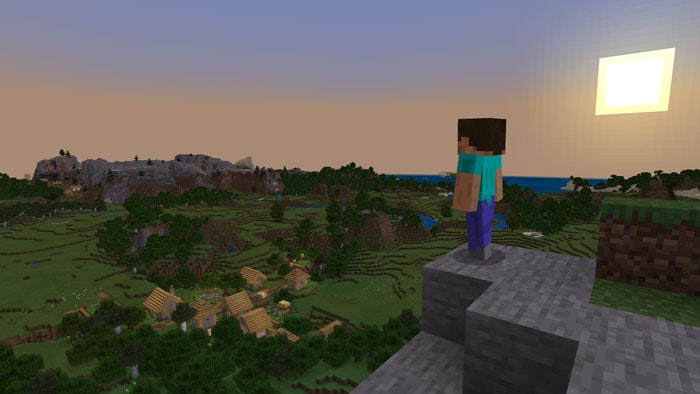
\includegraphics[width=8cm]{Images/InitialResearch/MCTerrainGeneration.png}}}
                        \qquad
                        \subfloat[\centering Example of a Sunken Pirate Ship Structure generated in the Game]{{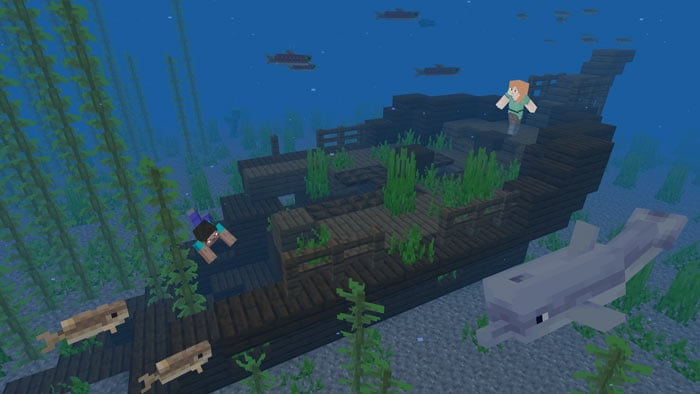
\includegraphics[width=8cm]{Images/InitialResearch/MCStructureGeneration.jpg}}}
                        \caption*{Promotional Imagery sourced from Minecraft.net}
                    \end{figure}

                    Minecraft itself is too complex and dynamic to be solved by current Machine Learning algorithms, along with there is no quantifiable 
                    metric for performance due to its sandbox nature. There exist data sets for Minecraft, in the form of captured gameplay footage, but
                    there has been little to no success of actually quantifiable good solutions to solving Machine Learning problems within Minecraft. \\

                    \vspace{0.2cm}

                    Overall I feel like it would be good to borrow elements from Minecraft's terrain generation, such as its utilization of Perlin Noise.
                    But the majority of the games systems are way too complex for a Machine Learning algorithm to solve. \\

                \paragraph{Conway's Game of Life} \mbox{} \\
                    \vspace{0.2cm}
                    Conway's Game of Life is what's called a Cellular Automaton, which is a discrete computation model formed from a grid of cells along with 
                    a rule set. Conway's is commonly referred to a Zero Player Game, where the input for the Automaton is defined at the start, with no
                    further adjustment needed for it to run. The game is fully Turing complete and can simulate a Universal Constructor. \\
                    \vspace{0.2cm}
                    The rules of Conway's are such that: \\

                    \vspace{0.2cm}
                    \begin{addmargin}[2em]{0em}
                        \large
                        1. Any live cell with fewer than two live neighbours dies, as if by underpopulation. \\
                        2. Any live cell with two or three live neighbours lives on to the next generation. \\
                        3. Any live cell with more than three live neighbours dies, as if by overpopulation. \\
                        4. Any dead cell with exactly three live neighbours becomes a live cell. \\
                    \end{addmargin}

                    \vspace{0.2cm}
                    It is rather interesting that such complicated Machines can be formed from such a simple rule set, as an example 
                    here is a Turing Machine formed from 34 Thousand Cells: \\

                    \begin{figure}[H]
                        \centering
                        \subfloat[\centering Turing Machine built in Conway's Game of Life]{{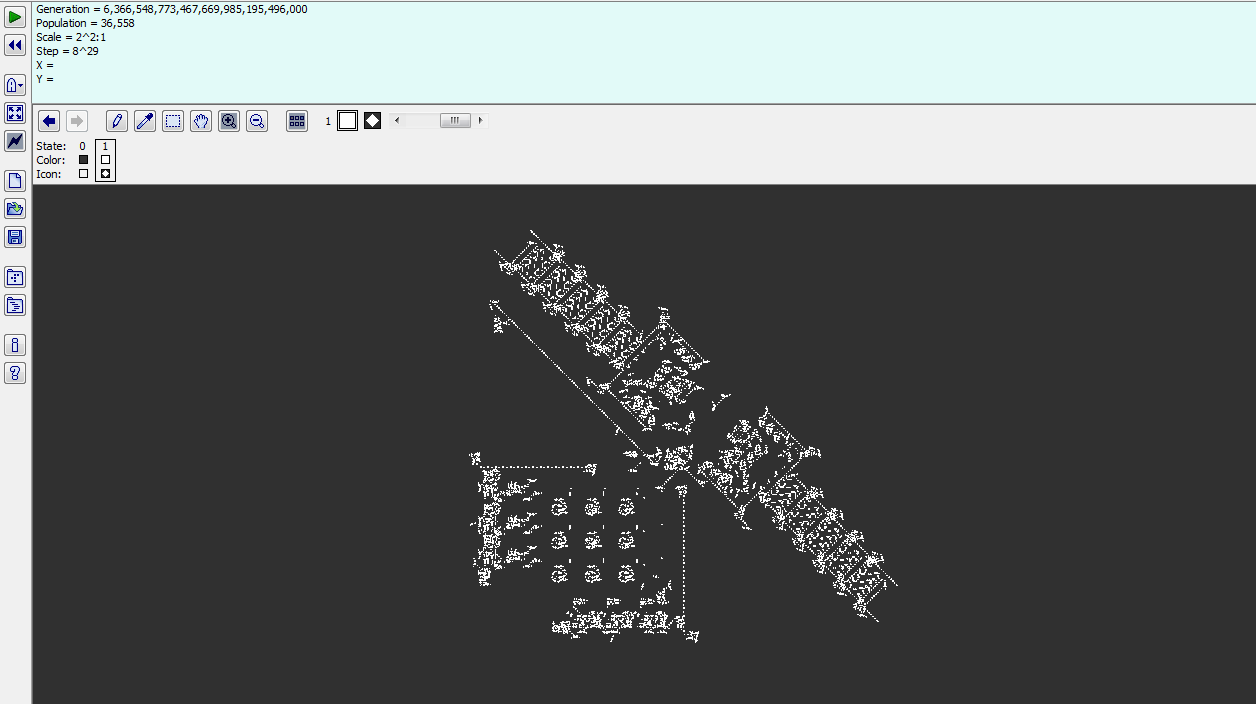
\includegraphics[width=14cm]{Images/InitialResearch/ConwaysTuringMachine.png}}}
                        \caption*{Sourced from Wikipedia}
                    \end{figure}

                    Overall, I think this shows that my simulation doesn't need to have complex rules in order to achieve 
                    interesting results. Conway's is formed from 4 simple rules, and yet is Turing complete.
            \subsubsection{Potential Algorithms/Data Types}
                \large
                \paragraph{Matrices} \mbox{} \\
                    If I go down the Neural Network Route, I will require a Matrix Implementation. Matrices store a grid of 
                    values which can have Arithmetic Operations performed on them like Addition and Multiplication. In the 
                    context of Machine Learning they can be used to speedup Operations significantly. They are commonly shown
                    like below. \\

                    \begin{center}
                        $\begin{bmatrix}
                            a & b\\
                            c & d
                        \end{bmatrix}$ 
                        $\begin{bmatrix}
                            a & b & c \\
                            d & e & f \\
                            g & h & i 
                        \end{bmatrix}$ 
                        $\begin{bmatrix}
                            a \\
                            b \\
                            c  
                        \end{bmatrix}$ 
                        $\begin{bmatrix}
                            a & b & c & d\\
                            e & f & g & h
                        \end{bmatrix}$ 
                    \end{center}   

                    They are a commonly implemented data type with well defined Operation Algorithms. If I didnt want to implement
                    it myself I could definitely find a library for the language I use which implements them for me.
                \paragraph{Neural Network} \mbox{} \\
                    Neural Networks are a key part of Machine Learning, and any complex enough algorithm to solve a procedurally 
                    generated environment will utilise one (see \textbf{Objective 5}). As part of my Initial Research I have taken the time to understand 
                    how a Neural Network functions, it turns out I have already learned most of the Maths needed to understand 
                    how it works in my A Level Maths and Further Maths courses. \\
                    \vspace{0.2cm}
                    A Neural Network functions as a series Mathematical Equations used to recognize relationships between inputs
                    and desired outputs. They take in a Vector of Input Data, and output a Vector of Output Data. They can be represented
                    in simple terms as a function: $N(x)$ where: $\{x \in V, N(x) \in V\}$.
                    The functions name in this case is Forward Propagation. \\
                    \vspace{0.2cm}
                    We form a Neural Network with multiple layers of Nodes, the layers being referred to as the Input Layer, 
                    Hidden Layer/s and Output Layer. In this case each Node is connected to every Node in the previous layer and
                    the following layer. In the below image is represented a Neural Network with a layer structure of $[3, 5, 2]$.

                    \begin{figure}[H]
                        \centerline{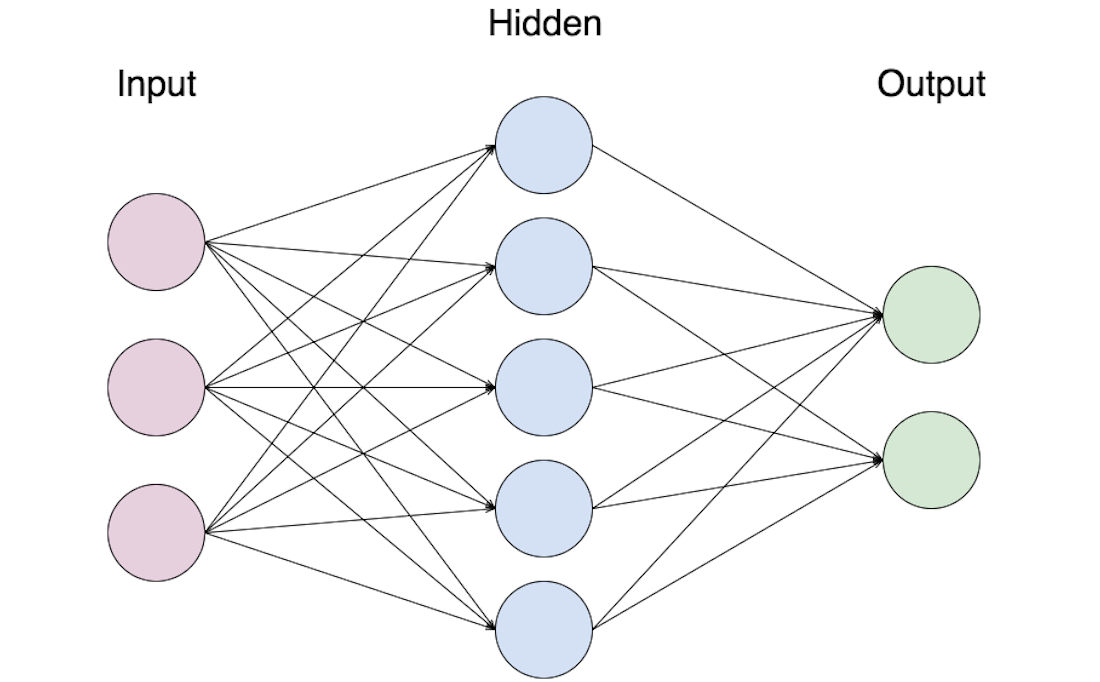
\includegraphics[width=10cm]{Images/InitialResearch/NeuralNetworkExample.png}}
                        \caption*{Sourced from https://webkid.io/blog/neural-networks-in-javascript/}
                    \end{figure}
                    

                    Each connection, otherwise known as an Arc or Edge, has an associated weight. Along with every output of a
                    layer having an associated Bias. These are used to compute the outcome of a network. \\
                    \vspace{0.2cm}
                    Forward Propagation is used to compute the outcome of a Network, it has a general form and uses 
                    Matrix Multiplication and Addition to achieve this.
                    \vspace{0.2cm}
                    
                    \begin{eqnarray*}
                        S^{(L)} &=& 
                        \begin{bmatrix}
                        s^{(L)}_{0} \\
                        s^{(L)}_{1} \\
                        \vdots      \\
                        s^{(L)}_{n} 
                        \end{bmatrix}
                        = 
                        \begin{bmatrix}
                        w^{(L-1)}_{0,0} & w^{(L-1)}_{0,1} & \hdots  & w^{(L-1)}_{0,m} \\
                        w^{(L-1)}_{1,0} & w^{(L-1)}_{1,1} & \hdots  & w^{(L-1)}_{1,m} \\
                        \vdots          & \vdots          & \ddots  & \vdots          \\
                        w^{(L-1)}_{n,0} & w^{(L-1)}_{n,1} & \hdots  & w^{(L-1)}_{n,m} \\
                        \end{bmatrix}
                        \begin{bmatrix}
                        a^{(L-1)}_{0} \\
                        a^{(L-1)}_{1} \\
                        \vdots      \\
                        a^{(L-1)}_{n} 
                        \end{bmatrix}
                        +
                        \begin{bmatrix}
                        b^{(L)}_{0} \\
                        b^{(L)}_{1} \\
                        \vdots      \\
                        b^{(L)}_{n} 
                        \end{bmatrix} \\
                        \sigma(S^{(L)}) &=& \sigma\left(
                        \begin{bmatrix}
                        s^{(L)}_{0} \\
                        s^{(L)}_{1} \\
                        \vdots      \\
                        s^{(L)}_{n} 
                        \end{bmatrix}
                        \right)
                        =
                        \begin{bmatrix}
                        \sigma(s^{(L)}_{0}) \\
                        \sigma(s^{(L)}_{1}) \\
                        \vdots              \\
                        \sigma(s^{(L)}_{n}) 
                        \end{bmatrix}
                    \end{eqnarray*}
                
                    \vspace{0.2cm}
                    We then apply an activation function as shown above, in this case we will apply the Sigmoid function: $\sigma(x)$ to $S^{(L)}$. 
                    The Sigmoid function is a Mathematical Function which \textit{squishes} values between 0 and 1. Shown Below:
                    
                    \begin{center}
                        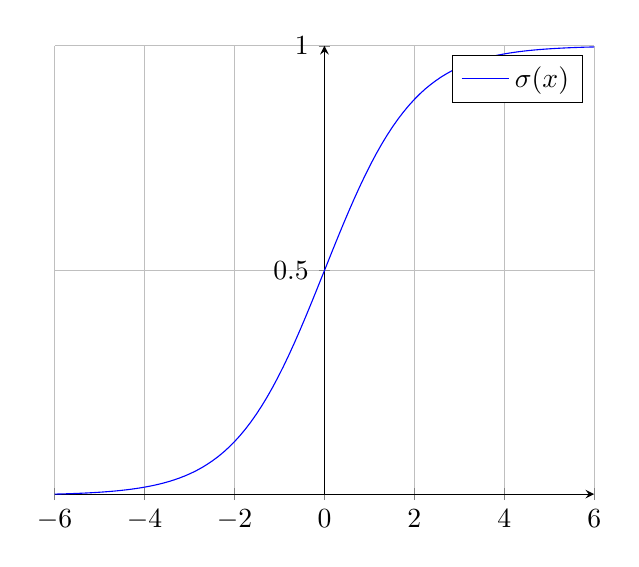
\begin{tikzpicture}[declare function={sigma(\x)=1/(1+exp(-\x));}]
                        \begin{axis}%
                        [
                            grid=major,     
                            axis x line=bottom,
                            ytick={0,.5,1},
                            ymax=1,
                            axis y line=middle,
                            samples=100,
                            domain=-6:6,
                            range=0:1
                            legend style={at={(1,0.9)}}     
                        ]
                            \addplot[blue,mark=none]   (x,{sigma(x)});
                            \legend{$\sigma(x)$}
                        \end{axis}
                        \end{tikzpicture}
                    \end{center}

                    Back Propagation is the opposite to Forward Propagation, and works by calculating the Derivaties (the Gradient Function) of each 
                    Weight and Bias within the Network. This is done with the Chain Rule and Multivariable Calculus. We then take this derivative away
                    from that specific Weight or Bias, eventually the Network will find a local minimum. This Process is called Gradient Descent.

                \paragraph{Q-Learning} \mbox{} \\
                    An alternative Algorithm I could use for my Machine Learning is Q-Learning. It is the step-down from utilising a Neural Network, so it is less 
                    complex in its Nature. It utilises the Bellman Equation, and something called a Q-Table. A Q table stores every possible state
                    the Agent could be in, and stores values for each action from the State. Every Action for every state has an initial value of 0 
                    and will be updated over time in order to "learn" the simulation. It is essentially a brute force method to Machine Learning. 
                    The greater the Value, the better the Q-Table will consider the action. Below is shown an example of a possible Q-Table I 
                    could use for my project:

                    \begin{center}
                        \begin{tabular}{ | c | c | c | c | c | c | c | c |}
                            \hline
                            \multicolumn{8}{|c|}{Q-Table} \\
                            \hline
                            \multicolumn{2}{|c|}{} & \multicolumn{6}{c|}{Actions} \\ 
                            \cline{3-8}
                            \multicolumn{2}{|c|}{} & North & East & South & West & Collect & Attack \\
                            \hline
                                    & 0     & 0 & 0 & 0 & 0 & 0 & 0 \\
                                    & \cdot & 0 & 0 & 0 & 0 & 0 & 0 \\
                            States: & \cdot & 0 & 0 & 0 & 0 & 0 & 0 \\
                                    & \cdot & 0 & 0 & 0 & 0 & 0 & 0 \\
                                    & N     & 0 & 0 & 0 & 0 & 0 & 0 \\
                            \hline
                        \end{tabular}
                    \end{center}

                    When trained extensively the Q-Table might start to look something like this:

                    \begin{center}
                        \begin{tabular}{ | c | c | c | c | c | c | c | c |}
                            \hline
                            \multicolumn{8}{|c|}{Q-Table} \\
                            \hline
                            \multicolumn{2}{|c|}{} & \multicolumn{6}{c|}{Actions} \\ 
                            \cline{3-8}
                            \multicolumn{2}{|c|}{} & North & East & South & West & Collect & Attack \\
                            \hline
                                    & 0     & \random & \random & \random & \random & \random & \random \\
                                    & \cdot & \random & \random & \random & \random & \random & \random \\
                            States: & \cdot & \random & \random & \random & \random & \random & \random \\
                                    & \cdot & \random & \random & \random & \random & \random & \random \\
                                    & N     & \random & \random & \random & \random & \random & \random \\
                            \hline
                        \end{tabular}
                    \end{center}
                    
                    I feel like the downside to this approach is that it will struggle to generalize to a procedurally generated simulation. If
                    given infinite time and infinite processing power it could theoretically solve anything, but sadly I don't have that kind of 
                    compute power. With the simulation I intend to design there would be to many Possible States for it to ever make a dent in.

                \paragraph{Procedural Generation} \mbox{} \\
                    For my project I am going to have to procedurally generate 2d terrain, while researching this I came across a few algorithms
                    which seemed to be able to do this pretty well. I will compare two algorithms I discovered below.
                    
                    \begin{center}
                        \begin{tabular}{| L{6cm} | L{6cm} |}
                            \hline
                            {\large Post-Processing Algorithms} & {\large Perlin Noise} \\
                            \hline
                            I discovered two post-processing algorithms often used for simple 2d terrain generation. 1 Averages squares 
                            around the selected square, and the other pulls it up or down the gradient its currently on.
                            I find these interesting because they're relatively simple, and I'm not quite sure whether they will produce good results or not. 
                            So it would be interesting to test out implementing these in my prototype.
                            &
                            Perlin Noise is an algorithm developed by Ken Perlin for use in the digital generation of noise.
                            This noise can be combined to create \textit{realistic} looking height maps for world generation.
                            Perlin Noise retains continuity and is seeded, so the generation can be entirely controlled.
                            By "retains continuity" I mean that you can sample the same point and retrieve the same value. 
                            If I was to implement Perlin noise it would take longer, but also might end up with a better result
                            due to it being more widely used. It's a trade-off between time to implement and desired result. \\
                            \hline
                        \end{tabular}
                    \end{center}
                    
                    I also discovered an algorithm called Poisson Disc Sampling, this can be used to sample random points 
                    in N dimensional space. It takes in 2 values, the R and K value, these values determine the output of
                    the function. The R values is the minimum distance a point has to be from another, randomly placed point
                    which hasn't been selected yet. If the distance between any existing points is less than R, the point
                    will be rejected and another will be selected. The K value determines how many rejected are needed before 
                    the algorithm will stop attempting to choose a new point.
        \subsection{Prototype}
            \subsubsection{Prototype Objectives}
            \large
            \vspace{0.2cm}
            Before starting my Prototype I had to decide upon a short list of objectives I wanted to 
            complete/investigate as part of it. These boiled down to a few things:

            \vspace{0.2cm}
            \begin{itemize}
                \item Terrain Generation
                \item Displaying the Generated Terrain using a Graphics Library
                \item Matrix and Vector implementation
            \end{itemize}
            \vspace{0.2cm}

            For my Prototype, I first created a GitHub Repository, available here: 
            
            \vspace{0.1cm}
            \centerline{\textit{https://github.com/TheTacBanana/CompSciNEAPrototype}}
            \vspace{0.1cm}

            I had created a hierarchy of importance for development in my head, visualized using this flow diagram:

            \begin{center}
                \begin{tikzpicture}
                    \matrix (m)[matrix of nodes, column  sep=0.5cm,row  sep=0.5cm, align=center, nodes={rectangle,draw, anchor=center} ]{
                        |[block]| Creating a window with Graphics Library &  |[block]| Display Generated Terrain \\   
                        |[block]| Generate Terrain using a pseudorandom algorithm &  |[block]| Store Terrain to 2d List \\
                        |[block]| Create a Matrix Data Structure & |[block]| Create a Vector Data Structure which inherits from Matrix \\
                        |[block]| Create Operation Methods for the Data Structure & \\
                    };
                    \path [>=latex,->] (m-1-1) edge (m-1-2);
                    \path [>=latex,<-] (m-1-2) edge (m-2-2);
                    \path [>=latex,->] (m-2-1) edge (m-2-2);
                    \path [>=latex,->] (m-3-1) edge (m-3-2);
                    \path [>=latex,->] (m-3-1) edge (m-4-1);
                \end{tikzpicture}
            \end{center}

            I decided to use Python for developing my Prototype, this seemed like a good fit due to me 
            having lots of experience with the language. Python is a Dynamically Typed and interpreted 
            which makes it versatile for prototyping and fast, iterative development.
            \subsubsection{Terrain Generation and Displaying to Window}
            Starting from the beginning of my hierarchy I installed Pygame using \textit{pip} and started creating a window.
            This was a relatively simple task only taking a few lines:
            \vspace{0.5cm}

            \normalsize
            \begin{pythoncode}
import pygame

simSize = 128
gridSize = 2

window = pygame.display.set_mode((simSize*gridSize, simSize*gridSize))
pygame.display.set_caption("Procedural Generation")

running = True
while running == True:
  for event in pygame.event.get():
    if event.type == pygame.QUIT:
      running = False
            \end{pythoncode}

            \vspace{0.5cm}

            \large
            This creates a window like this: \\ 
            \vspace{0.5cm}
            \centerline{
\includegraphics{Images/Prototype/CreateWindowExample.PNG}}

            \vspace{0.5cm}

            Following the hierarchy I then added noise generation by generating random numbers and 
            assigning them to a 2d List. Shown here: 
            
            \begin{pythoncode}
def GenerateMap(self, seed):
    random.seed(seed)
    for y in range(0, self.arraySize):
        for x in range(0, self.arraySize):
            self.heightArray[x][y] = round(random.random(),2)
        \end{pythoncode}

            \vspace{0.5cm}

            \large
            After creating some code to draw squares based upon the random value, I ended up with this 
            random array of Black-White squares:\\
            \vspace{0.5cm}
            \centerline{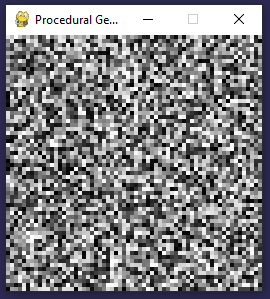
\includegraphics{Images/Prototype/RandomNoiseExample.PNG}}

            \vspace{0.5cm}

            This was a good start, but didn't really look like terrain yet. As part of my research I came 
            across simple algorithms to turn random noise into usable 2d terrain. I decided to implement
            these algorithms. They are relatively short and didn't take too much time to implement. I've
            named the two algorithms UpDownNeutralGen and Average.

            \vspace{1cm}

            \paragraph{UpDownNeutralGen Method} \mbox{} \\
            \vspace{0.25cm}

            The UpDownNeutralGen method takes a tile, and considers every tile around it. It sums the tile 
            which are greater than, less than, or within a certain range of the tile height. And then pulls
            the selected tile in the direction which has the highest precedence. As an example, here are some
            randomly generated values:

            \begin{center}
                \begin{tabular}{| C{0.75cm} | C{0.75cm} | C{0.75cm} |}
                    \hline
                    0.71 & 0.19 & 0.3 \\ [0.75cm]
                    \hline
                    0.46 & 0.26 & 0.82 \\ [0.75cm]
                    \hline
                    0.63 & 0.35 & 0.05 \\ [0.75cm]
                    \hline
                \end{tabular}
            \end{center}

            If we count the surrounding values into corresponding Higher, Lower and Neutral we get: \\

            \begin{center}
                \begin{tabular}{| M{2cm} | M{2cm} | M{2cm} |}
                    \hline
                    Higher & Lower & Neutral \\ [0.25cm]
                    \hline
                    4 & 1 & 3 \\ [0.25cm]
                    \hline
                \end{tabular}
            \end{center}

            \vspace{0.5cm}

            This leads us to calculating the \textit{pullValue}, respectively for each case:
            \begin{eqnarray*}
                \text{pullValue } &=& 
                \begin{cases}
                    \text{upTiles} \times 0.09 & \text{Most Up Tiles} \\
                    \text{downTiles} \times -0.08 & \text{Most Down Tiles} \\
                    0 & \text{Most Neutral Tiles} 
                \end{cases} \\
                \text{Value}[x][y] &=& \text{pullValue}
            \end{eqnarray*}
            
            \vspace{0.5cm}

            We then add the pullValue to the original square value, leaving us with the updated value.
            The code for this is shown below:
            \begin{pythoncode}
def UpNeutralDownGen(self):
    dupMap = self.heightArray
    for y in range(0, self.arraySize):
        for x in range(0, self.arraySize):
            up = 0
            down = 0
            neutral = 0
            pointArr = []

            if x != 0 and y != 0:
                pointArr.append(self.heightArray[x - 1][y - 1])
            if x != 0 and y != self.arraySize - 1:
                pointArr.append(self.heightArray[x - 1][y + 1])
            if x != self.arraySize - 1 and y != self.arraySize - 1:
                pointArr.append(self.heightArray[x + 1][y + 1])
            if x != self.arraySize - 1 and y != 0:
                pointArr.append(self.heightArray[x + 1][y - 1])
            if x != 0:
                pointArr.append(self.heightArray[x - 1][y])
            if y != 0:
                pointArr.append(self.heightArray[x][y - 1])
            if x != self.arraySize - 1:
                pointArr.append(self.heightArray[x + 1][y])
            if y != self.arraySize - 1:
                pointArr.append(self.heightArray[x][y + 1])

            for i in range(len(pointArr)):
                if pointArr[i] >= self.heightArray[x][y] + 0.1:
                    up += 1
                elif pointArr[i] <= self.heightArray[x][y] - 0.1:
                    down += 1
                else:
                    neutral += 1

            if (up > down) and (up > neutral): # Up
                value = 0.09 * up
            elif (down > up) and (down > neutral): # Down
                value = -0.08 * down
            else: # Neutral
                value = 0

            dupMap[x][y] += value
            dupMap[x][y] = self.Clamp(dupMap[x][y], 0, 1)

    self.heightArray = dupMap
            \end{pythoncode}

            \paragraph{Average Method} \mbox{} \\
            \vspace{0.25cm}

            The Average method takes a tile and considers every tile around it, this time instead of looking at the
            differences, it creates an average from the 8 surrounding tiles. It then sets the selected tile to this
            average value. As an example, here are some randomly generated values:

            \begin{center}
                \begin{tabular}{| C{0.75cm} | C{0.75cm} | C{0.75cm} |}
                    \hline
                    0.83 & 0.93 & 0.64 \\ [0.75cm]
                    \hline
                    0.07 & 0.38 & 0.21 \\ [0.75cm]
                    \hline
                    0.33 & 0.94 & 0.95 \\ [0.75cm]
                    \hline
                \end{tabular}
                \vspace{0.25cm}

                Summing these and dividing by the total amount of tiles grants us the average:

                \begin{eqnarray*}
                    \frac{0.83 + 0.93 + 0.64 + 0.07 + 0.38 + 0.21 + 0.95 + 0.33 + 0.94}{9} &=& 0.586 \\
                    Value[x][y] &=& 0.586
                \end{eqnarray*}
            \end{center}
            \vspace{0.25cm}

            The code for this is shown below:
            \begin{pythoncode}
def AverageGen(self):
    dupMap = self.heightArray
    for y in range(0, self.arraySize):
        for x in range(0, self.arraySize):        
            total = 0
            count = 0
            if x != 0 and y != 0:
                total += self.heightArray[x - 1][y - 1]
                count += 1
            if x != 0 and y != self.arraySize - 1:
                total += self.heightArray[x - 1][y + 1]
                count += 1
            if x != self.arraySize - 1 and y != self.arraySize - 1:
                total += self.heightArray[x + 1][y + 1]
                count += 1
            if x != self.arraySize - 1 and y != 0:
                total += self.heightArray[x + 1][y - 1]
                count += 1
            if x != 0:
                total += self.heightArray[x - 1][y]
                count += 1
            if y != 0:
                total += self.heightArray[x][y - 1]
                count += 1
            if x != self.arraySize - 1:
                total += self.heightArray[x + 1][y]
                count += 1
            if y != self.arraySize - 1:
                total += self.heightArray[x][y + 1]
                count += 1

            dupMap[x][y] = total / count
    self.heightArray = dupMap
            \end{pythoncode}
            \subsubsection{Finished Terrain Generation}
            \vspace{0.25cm}

            Overall I am happy with the Terrain generation, though I feel as if it could be improved to look more realistic.
            Though I do think the difference between the original random noise and the Colour Mapped Terrain looks so much better. I
            think utilising Perlin Noise in my Project would be a better option (see \textbf{Objective 4.2.2})

            \begin{figure}[h]
                \centering
                \subfloat[\centering Greyscale Terrain Generation]{{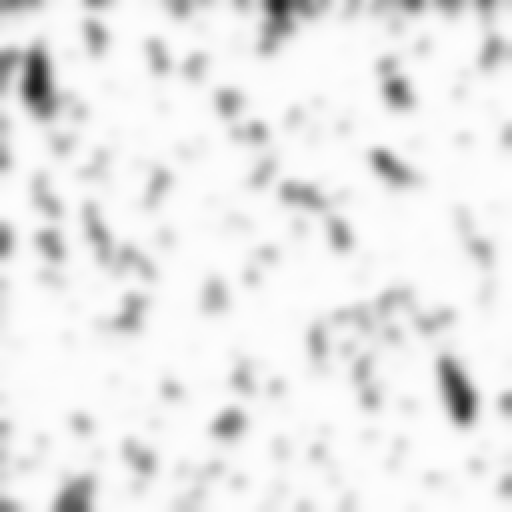
\includegraphics[width=6cm]{Images/Prototype/Seed420 Grayscale.png}}}
                \qquad
                \subfloat[\centering Colour Bands applied to the Terrain Generation]{{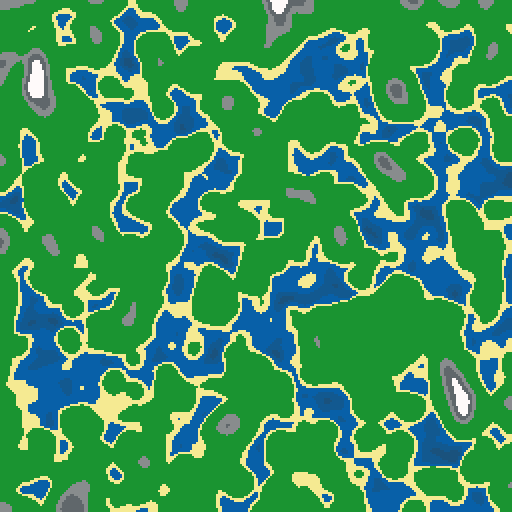
\includegraphics[width=6cm]{Images/Prototype/Seed420 Colour.png} }}
            \end{figure}
            \subsubsection{Matrix Data Structure}
                \vspace{0.25cm}

                As part of my Matrix Class I made a list of operations which would be key to a Matrix Class, along with being useful
                for Machine Learning. A Matrix is an abstract data type, commonly used in Maths, but has practical uses in the world
                of Computer Science. It holds a 2d array of values such as: \\ 
                \begin{center}
                $\begin{bmatrix}
                    a & b\\
                    c & d
                \end{bmatrix}$ 
                $\begin{bmatrix}
                    a & b & c \\
                    d & e & f \\
                    g & h & i 
                \end{bmatrix}$ 
                $\begin{bmatrix}
                    a \\
                    b \\
                    c  
                \end{bmatrix}$ 
                $\begin{bmatrix}
                    a & b & c & d\\
                    e & f & g & h
                \end{bmatrix}$ 
                \end{center}
                The values in a Matrix can be manipulated using common operations such as $+ - *$ as long as the orders of the 2 Matrices
                match up. Along with other, non-standard operations which have other purposes.

                \vspace{0.25cm}
                As part of my Matrix Class, I implemented the following operators:
                \begin{enumerate}
                    \item Addition/Subtraction \\
                        Implementing Addition didn't take too long, I utilised a nested for loop to iterate over every value in both Matrices.
                        Adding the two values together into a temporary Matrix which the method then returned. 
                        \vspace{0.25cm}
                        \begin{center}
                            $\begin{bmatrix}
                                a & b\\
                                c & d
                            \end{bmatrix} +
                            \begin{bmatrix}
                                e & f\\
                                g & h
                            \end{bmatrix} =
                            \begin{bmatrix}
                                a+e & b+f\\
                                c+g & d+h
                            \end{bmatrix}$
                        \end{center}
                        \vspace{0.25cm}

                        The written code is shown below:
                        \begin{pythoncode}
@staticmethod
def MatrixAddSubtract(m1, m2, subtract = False):
    m1Dims = m1.Dimensions()
    newMat = Matrix(m1Dims[0], m1Dims[1])
    for y in range(0, m1Dims[0]):
        for x in range(0, m1Dims[1]):
            if subtract:
                newMat.matrixArr[y][x] = m1.Val()[y][x] - m2.Val()[y][x]
            else:
                newMat.matrixArr[y][x] = m1.Val()[y][x] + m2.Val()[y][x]
    return newMat
                        \end{pythoncode}

                    \item Multiplication \\
                        Multiplication of Matrices is slightly more complicated, it is of $O(n^3)$ complexity, utilising a triple nested for loop.
                        It multiplies the row of a $M1$, by the column in $M2$. Summing the calculation into the element in the new Matrix $M3$. \\
                        
                        \vspace{0.25cm}
                        \begin{center}
                            $\begin{bmatrix}
                                a & b\\
                                c & d
                            \end{bmatrix} \times
                            \begin{bmatrix}
                                e & f\\
                                g & h
                            \end{bmatrix} =
                            \begin{bmatrix}
                                a*e + b*g & a*f + b*h\\
                                c*e + d*g & c*f + d*h
                            \end{bmatrix}$
                        \end{center}
                        There is also Scalar Multiplication which multiples each value of a Matrix by the Scalar.
                        \begin{center}
                            $k *
                            \begin{bmatrix}
                                a & b\\
                                c & d
                            \end{bmatrix} =
                            \begin{bmatrix}
                                ka & kb\\
                                kc & kd
                            \end{bmatrix}$
                        \end{center}
                        \vspace{0.25cm}

                        The written code is shown below:
                        \begin{pythoncode}
@staticmethod                        
def ScalarMultiply(s, m1):
    m1Dims = m1.Dimensions()
    newMat = Matrix(m1Dims[0], m2Dims[1])
    for y in range(0, m1Dims[0]):
        for x in range(0, m1Dims[1]):
            newMat.matrixArr[y][x] = m1.matrixArr[y][x] * s

@staticmethod
def MatrixMultiply(m1, m2):
    m1Dims = m1.Dimensions()
    m2Dims = m2.Dimensions()
    newMat = Matrix(m1Dims[0], m2Dims[1])
    for row in range(0, m1Dims[1]):
        subRow = m1.Val()[row][0:m1Dims[1]]
        for col in range(0, m2Dims[1]):
            subCol = []
            for i in range(0, m1Dims[0]):
                print(i)
                subCol.append(m2.Val()[i][col])
            total = 0
            for x in range(0, len(subRow)):
                total += subRow[x] * subCol[x]
            newMat.matrixArr[row][col] = total
    return newMat
                        \end{pythoncode}

                    \item Determinant \\
                        Calculating the Determinant of an $nxn$ Matrix is a recursive algorithm. With the base case being the Determinant of a 2x2
                        Matrix. When calculating the Determinant of a 3x3 Matrix you create a Matrix of Cofactors, and multiply each 
                        value by the corresponding value in the Sin Matrix (\textit{Formed from repeating 1's and -1's}). Summing the values from
                        a singular Row or Column will then give you the Determinant. For a 4x4 you simply calculate the Determinant of the corresponding
                        3x3's to get the Cofactors.
                        
                        \begin{center}
                            $
                            \begin{vmatrix}
                                a & b\\
                                c & d
                            \end{vmatrix} = 
                                a*d - b*c
                            $
                        \end{center}
                        \vspace{0.25cm}
                        \begin{center}
                            $\begin{vmatrix}
                                a & b & c \\
                                d & e & f \\
                                g & h & i 
                            \end{vmatrix}  = a*
                            \begin{vmatrix}
                                e & f\\
                                h & i
                            \end{vmatrix}
                            -b*
                            \begin{vmatrix}
                                d & f\\
                                g & i
                            \end{vmatrix}
                            +c*
                            \begin{vmatrix}
                                d & e\\
                                g & h
                            \end{vmatrix}$
                        \end{center}
                        \vspace{0.25cm}

                        The written code is shown below:
                        \begin{pythoncode}
def SubMatrixList(self, rowList, colList):
    newMat = Matrix(self.Dimensions()[0] - len(rowList),self.Dimensions()[1] - len(colList))
    xoffset = 0
    yoffset = 0
    yRowList = []

    for y in range(0, self.Dimensions()[0]):
        for x in range(0, self.Dimensions()[1]):
            if x in colList and y in rowList:
                xoffset += 1
                yoffset += 1
                continue
            elif x in colList:
                xoffset += 1
                continue
            elif y in rowList and y not in yRowList:
                yoffset += 1
                yRowList.append(y)
                continue
            else:
                newMat.matrixArr[y - yoffset][x - xoffset] = self.matrixArr[y][x]
        xoffset = 0
    return newMat

@staticmethod
def Determinant(m):
    dims = m.Dimensions()
    if dims[1] <= 2:
        det = (m.matrixArr[0][0] * m.matrixArr[1][1]) - (m.matrixArr[0][1] * m.matrixArr[1][0])
        return (det)
    elif dims[1] != 2:
        det = 0
        subtract = False
        tempMat = m.SubMatrixList([0],[])
        for i in range(0, dims[1]):
            subMat = None
            subMat = m.SubMatrixList([0],[i])
            if subtract == False:
                det += m.matrixArr[0][i] * Matrix.Determinant(subMat)
                subtract = True
            elif subtract == True:
                det -= m.matrixArr[0][i] * Matrix.Determinant(subMat)
                subtract = False
        return det
                        \end{pythoncode}

                    \item Dot Product \\
                        The Dot Product occurs between two vectors, and can be used to calculate the angle between them. 
                        It's a relatively simple operation only taking a few lines of code.
                        \begin{center}
                            $
                            \begin{bmatrix}
                                a \\
                                b \\
                                c
                            \end{bmatrix} .
                            \begin{bmatrix}
                                d \\
                                e \\
                                f
                            \end{bmatrix} = 
                            a \times d + b \times e + c \times f$
                        \end{center}
                        \vspace{0.25cm}

                        The written code is shown below:
                        \begin{pythoncode}
@staticmethod
def DotProduct(v1,v2):
    total = 0
    for i in range(v1.Dimensions()[0]):
        total += v1.Val()[i][0] * v2.Val()[i][0]
    return total
                        \end{pythoncode}
                \end{enumerate}
            \subsubsection{Prototype Evaluation}
                \vspace{0.2cm}
                Overall I am happy with my prototype, though I feel like it needs improvement. I did meet my 
                objectives for my prototype, but there are things I want to change for my Technical Solution. 
                The Terrain Generation along with the Matrix class. I feel that Perlin noise would be a better alternative
                to the two algorithms I used (see \textbf{Objective 4.2.2}). In theory, it should produce better results, and also provide more marks for 
                complexity. My Matrix Class could also be rewritten to be more efficient (see \textbf{Objective 3.9}), my implementation of the Operations is not the best.
                I also feel like having Vector inherit from Matrix is relatively pointless, there is no need for it when I could just use 
                1 wide Matrices instead.
        \subsection{Further Research}
            \subsubsection{Second Interview}
                I asked a few more questions to my Expert regarding my project at this point. Receiving feedback on my Prototype and gaining a
                greater understanding of the Machine Learning Model I'm intending to use. \\
                \vspace{0.2cm}

                \begin{enumerate}
                    \item What are your thoughts on my prototype? \\ 
                        \vspace{0.2cm}
                        "I think your prototype is good, but could be improved. The use of Operator Overloading would improve your Matrix Class,
                        and optimizing some of your algorithms would be useful. The Terrain generation looks good, but I think it's a bit
                        water heavy, this is where Perlin Noise might help you to achieve better results. Would also be more fine tunable to
                        your liking."

                    \item Is a Dual Neural Network a good model to choose? \\
                        \vspace{0.2cm}
                        "A Dual Neural Network should in theory be a complex enough Model for your project. The concern I have is whether your
                        Network will be able to generalize enough in order to sufficiently 'solve' the simulation you design. There are some
                        algorithms you could implement in order to tackle this though. You could do some research into these before finalizing 
                        your design."

                    \item Is an Object Orientated Network a good approach? \\
                        \vspace{0.2cm}
                        "Implementing your Network using a Class hierarchy would allow you to organize your code nicely, passing objects between
                        methods. With a Dual Neural Network you could create two instances of a Network class using them as your Main and Target 
                        Network. This would also gain your marks for coding style."

                    \item Which Activation Functions should I implement? \\
                        \vspace{0.2cm}
                        "The most commonly used are Sigmoid, TanH, ReLu and SoftMax. They are relatively simple so won't take long to implement.
                        Those would be a good starting point for testing your Neural Network."
                    
                    \item What type of Reward Structure should I use? \\
                        \vspace{0.2cm}
                        "As far as I'm aware there are two types of Reward Structures, Sparse and Dense. I think that Dense would be better suited
                        to your project. Sparse is where the reward given to the Agent is 0 for most actions. Compared to dense where reward
                        is given for most actions. Say if you want to motivate exploration I feel like dense would be appropriate."

                    \item What type of pathfinding should I use for the Enemies in my Simulation? \\
                        \vspace{0.2cm}
                        "I don't think it would be necessary to implement any complex algorithm for your Enemies Pathfinding, it will only eat 
                        into your performance when training the Network. But if you do want to implement a complex algorithm, Dijkstra's or A* Search 
                        would be appropriate."
                \end{enumerate}
            \subsubsection{Evaluation of Second Interview}
                My Expert's feedback has been useful in this case. Below is my thoughts on various parts of the Interview:
                
                \begin{itemize}
                    \item I am in agreement with him about my prototype, it really has a lot of improvements to be made. Shaun mentioned Operator 
                    overloading which I was unaware Python could utilise at the time of creating my Matrix Class, I will definitely use this in 
                    my Technical Solution (see \textbf{Objective 3.8}). 

                    \item I will definitely be implementing a Dual Neural Network then (see \textbf{Objective 5}). He shared his concerns about its ability to solve complex 
                    problems of this Nature. Due to the nature of my project, this will be fine as I'll still be able to analyse the Algorithms Results.
                    The results will hopefully show a declining trend in Network Loss.

                    \item I will be using an Object Orientated Model for my Program, so I feel like this is the best way forward. His suggestion 
                    about the two instances of Network for Main and Target will be useful (see \textbf{Objective 5.1}).

                    \item Encouraging exploration is something I definitely want to do, so I will try to implement a Dense Reward Structure.
                    
                    \item I didn't have any plans to implement a complex path finding algorithm, so this is helpful to see we're in agreement.

                \end{itemize}
            \subsubsection{Research Material}
                As part of my Further Research, I did more research relating to specific parts of my project. These are listed below along with 
                descriptions about their contents and what I've gained from them:
                
                \paragraph*{Playing Atari with Deep Reinforcement Learning - DeepMind} \mbox{} \\
                    This paper contained helpful information regarding the Deep Q Learning Algorithm, allowing me to gain a deeper understanding
                    of how it works. The main goal of this Paper was to train an Algorithm to play Atari Games through using raw pixel data. They
                    manage to achieve relatively good results, with the Average Reward per Epoch and Average Action Value showing positive
                    trends for the tested games.

                \paragraph*{Revisiting Fundamentals of Experience Replay - DeepMind} \mbox{} \\        
                    This Paper defines the Experience Replay Algorithm in use with Deep Q Networks. It allowed me to gain an insightful understanding
                    into the motivations behind how the Algorithm works. It also outlines a process for Prioritized Experience Replay, but I did not
                    end up using this as part of my project.

                \paragraph*{Benchmarking the Spectrum of Agent Capabilities - Google Research} \mbox{} \\
                    I read this Paper as part of my Initial Research. It was interesting to see something so similar to my Project being researched
                    at a higher level. The problems they struggled which I outlined in my Existing Investigations Section informed some of my simulation
                    design, in an attempt to Mitigate the problems they face.

                \paragraph*{Fast Poisson Disc Sampling in Arbitrary Dimensions - Robert Bridson} \mbox{} \\
                    This Paper outlines the Algorithm used for Poisson Disc Sampling in detail. There is not much else to it. I saved it for later
                    for when I come to implementing it in my Technical Solution.

                \paragraph*{Neural Networks - 3Blue1Brown} \mbox{} \\
                    This is a helpful video series designed to explain Neural Networks from a ground up point of view. It goes through all the Maths
                    in a comprehensive way, which I found very helpful when trying to get my head around Back Propagation. Having a video series I
                    can rewatch over and over was helpful in this process.

                \paragraph*{Mathematics of Backpropagation - Brian Dolhansky} \mbox{} \\
                    This article about Back Propagation was very helpful when trying to find a general form for Matrix Back Propagation. Its lays
                    out Neural Networks from an easy-to-follow standpoint, making it easier for me to find my own General Matrix Form, shown in
                    Modelling of the Problem. 
        \subsection{Objectives}
            \large
            Taking into account my Prototype and Interviews, I have formed a list of objectives I feel to be most 
            appropriate for my Investigation. If all completed they will form a complete solution which will answer 
            my Investigations question.\\

            \renewcommand{\labelenumii}{\arabic{enumi}.\arabic{enumii}}
            \renewcommand{\labelenumiii}{\arabic{enumi}.\arabic{enumii}.\arabic{enumiii}}
            \renewcommand{\labelenumiv}{\arabic{enumi}.\arabic{enumii}.\arabic{enumiii}.\arabic{enumiv}}

            \begin{enumerate}
                \item The Program must have User Input
                \begin{enumerate}
                    \item Before Launching the Program the User should be able to adjust individual Parameters of the Program
                    \item Examples of such Parameters are:
                    \begin{enumerate}
                        \item World Size
                        \item Tile Colour Values
                        \item Neural Network Layer Size
                    \end{enumerate}
                    \item These Parameters should be stored in a User Readable File/Plain Text
                    \item These Parameters should be checked against Ranges before being used in the Program
                    \item These Ranges should be specified in a separate File
                    \item An Error message should be displayed if a Parameter is Out of Range
                    \item The User should be prompted to load previous Training Data from a File
                \end{enumerate}

                \item The Program must have Graphical Output
                \begin{enumerate}
                    \item After User input is complete a Graphical Window should open
                    \item This Window should display the current state of the simulation
                    \item The Agent should be displayed to the Window
                    \item The Enemies should be displayed to the Window
                    \item The Objects should be displayed to the Window
                    \item The Window should display each element with its correct Colour
                    \item When enabled a Debug Side Bar should be displayed
                    \item The Debug Side Bar should the Neural Networks Activation Values
                \end{enumerate}

                \item The Program must contain a Matrix Implementation
                \begin{enumerate}
                    \item Data for the Matrix must be stored in a 2d List/Array
                    \item A Property must exist for the order of the Matrix
                    \item Multiple initialization Methods must be possible
                    \begin{enumerate}
                        \item Creation using a Tuple of Integers
                        \item Creation using an existing 2d List
                        \item Creation using an existing 1d List
                    \end{enumerate}
                    \item It must be possible to fill a Matrix with Randomized Values
                    \item It must be possible to create the Identity Matrix of N Size
                    \item There should be a way to print a Matrix to the Console
                    \item There should be Methods for Standard Matrix Operations
                    \begin{enumerate}
                        \item Addition 
                        \item Subtraction
                        \item Multiplication
                        \item Scalar Multiplication
                        \item Hadamard Product
                        \item Transpose
                        \item Sum
                    \end{enumerate}
                    \item Most of these Operations should utilise Operator Overloading where possible
                    \item The Operations should be implemented utilising Efficient Algorithms (Minimised Time Complexity)
                    \item Appropriate Error messages should be in place when utilising Matrices incorrectly
                \end{enumerate}

                \item The Program must contain an Agent and Simulation Environment
                \begin{enumerate}
                    \item The Simulation Environment must be stored in a WorldMap Object 
                    \item The Simulation Environment must be Procedurally Generated
                    \begin{enumerate}
                        \item The Simulation Environment must be generated using a Seed
                        \item The Terrain must be Generated utilising the Perlin Noise Algorithm
                        \item The Terrain Data must be Stored in Tile Objects
                        \item Each Tile Object must be assigned Tile Type based on its Height Value
                        \item Each Tile Type must use a Colour Specified by the User
                        \item Objects must be placed around the Environment for the Agent to Collect
                        \item The Objects must be placed utilising the Poisson Disc Sampling Algorithm
                        \item Enemies must be randomly placed around the Environment at the start of a World
                        \item The Enemies must path find towards the Agent
                    \end{enumerate}
                    \item The Simulation must have Finite State Transitions
                    \item The Agent must be spawned into the Simulation
                    \item The Agent must be controlled by the Machine Learning Algorithm
                    \item The Agent must have a Finite Action Set
                    \item The Agent must have a Position which can be altered by its Actions
                    \item The Agent must be able to Pick up Items
                    \item Any Collected Items must be stored in the Agents Inventory
                    \item The Agent must be able to Attack Enemies
                    \item The Agent must be able to be killed by the Enemies
                    \item The Agent should be killed when it traverses into Water
                    \item When the Agent is killed the Simulation should Reset
                    \item The Agent must have a Reward Structure
                    \begin{enumerate}
                        \item The Agent must gain Reward from doing specific things
                        \item Reward must be gained from exploration
                        \item Reward must be gained from Killed an Enemy
                        \item Reward must be gained from Collecting an Item
                        \item Reward must be lost from Dying
                        \item Reward must be lost from Failing an Attack
                    \end{enumerate}
                    \item When the Simulation is reset the Terrain should be Procedurally Generated again
                    \item When the Simulation is reset the Objects should be placed again
                    \item When the Simulation is reset the Enemies should be spawned again
                    \item When the Simulation is reset the Agent should be spawned again
                    \item The Agent must be able to Sample its Environment for Tile Data
                    \item This Tile Data must be able to be converted into Greyscale Values
                    \item These Greyscale Values must be used as the Neural Networks Input
                \end{enumerate}

                \item The Program must contain a Dual Neural Network
                \begin{enumerate}
                    \item The Dual Neural Network must be formed from two instances of a Neural Network Class
                    \begin{enumerate}
                        \item The Neural Network must be implemented utilising an Object Orientated Model
                        \item The Neural Network must contain Forward Propagation
                        \item The Neural Network must utilise the Bellman Equation to find Expected Values
                        \item The Expected Values must be used when Calculating the Loss of the Network
                        \item The Neural Network must contain Backwards Propagation
                        \item The Back Propagation must utilise the Calculated Loss when calculating the Error Signal
                        \item The Forward and Back Propagation must be Implemented utilising Matrix Operations
                        \item The Neural Network must be able to utilise Activation Functions
                    \end{enumerate}
                    \item The Target Network must be updated intermittently
                    \item The Neural Network must be Trainable by inputting collected Greyscale Values
                    \item The Agent must collect these Greyscale Values
                    \item The Neural Network should instruct the Agents Actions
                    \item The Neural Network should utilise the Epsilon Greedy decision process
                    \item The Neural Network should utilise the SoftMax Function when picking an Action
                    \item The Neural Network should utilise Experience Replay
                    \item Each State should be stored in an Experience Object
                    \item Experience Replay should be performed intermittently
                    \item The Training Data must be able to be Saved as .dqn Files
                    \item Experience Replay States should be stored in a Double Ended Queue
                \end{enumerate}

                \item The Program must contain Activation Functions
                \begin{enumerate}
                    \item The Activation Functions must be used within the Dual Neural Network
                    \item An Activation Function must be defined as an Abstract Base Class
                    \item An Activation Function must have a Normal and Derivative Method
                    \item An Activation Function must take a Vector as an Input
                    \item An Activation Function must return a Vector as an Output
                    \item There must be standard Activation Functions implemented
                    \begin{enumerate}
                        \item Sigmoid
                        \item TanH
                        \item ReLu
                        \item Leaky ReLu
                    \end{enumerate}
                \end{enumerate}

                \item The Program must contain a Data Logger
                \begin{enumerate}
                    \item The Data Logger must use a specific Structure
                    \item When adding a Data Point it must match the Data Loggers Structure
                    \item If it does not it should display an Error Message
                    \item The Data Points should be saved to a .data File
                    \item The Data Logger must contain a Heap Sort to find minimum and maximum values
                    \item The Heap Sort must allow sorting via an index of the Data Point
                    \item The Heap Sort must utilise an Efficient Algorithm (Minimized Time Complexity)
                \end{enumerate}

                \item The Program must contain a Script to Graph Data
                \begin{enumerate}
                    \item The Script must present the User options for which .data file to plot
                    \item The Script must present the User options for which part of the Data to Plot
                    \item The Script must display a graph of the data
                \end{enumerate}
            \end{enumerate}
        \subsection{Modelling of the Problem}
            \large
            In this section I will define and derive all the Mathematical Formulae relating to my Project. This includes all the Matrix Operations 
            I plan to use and the General Forms of Forward Propagation and Back Propagation. \\

            \subsubsection{Matrices}
                \paragraph{Overview} \mbox{} \\
                Matrices are a Mathematical Data Structure, storing elements in the shape of a Rectangle. They are arranged Rows and Columns.
                An $m$ x $n$ Matrix will have $m$ Rows and $n$ Columns. This is being modelled to fulfil \textbf{Objective 3}.\\
                \vspace{0.2cm}
                As part of defining the Matrix Operations, below is defined Matrix $A$ and Matrix $B$ and can be of any size. \\
                \vspace{0.5cm}

                \begin{center}
                    $
                    A = 
                    \begin{bmatrix}
                        a_{1,1} & a_{1,2} & \hdots  & a_{1,m} \\
                        a_{2,1} & a_{2,2} & \hdots  & a_{2,m} \\
                        \vdots  & \vdots  & \ddots  & \vdots  \\
                        a_{n,1} & a_{n,2} & \hdots  & a_{n,m} \\
                    \end{bmatrix}
                    $
                \end{center}
                \vspace{0.2cm}
                \begin{center}
                    $
                    B = 
                    \begin{bmatrix}
                        b_{1,1} & b_{1,2} & \hdots  & b_{1,m} \\
                        b_{2,1} & b_{2,2} & \hdots  & b_{2,m} \\
                        \vdots  & \vdots  & \ddots  & \vdots  \\
                        b_{n,1} & b_{n,2} & \hdots  & b_{n,m} \\
                    \end{bmatrix}
                    $
                \end{center}

                \paragraph{Matrix Addition} \mbox{} \\
                    \vspace{0.2cm}
                    Matrix Addition is the Operation of adding two Matrices by adding the Corresponding Elements together. Matrix Addition is Commutative. 
                    Below is A added to B. (See \textbf{Objective 3.7.1}.\\

                    \begin{center}
                        $
                        A + B =
                        \begin{bmatrix}
                            a_{1,1} + b_{1,1} & a_{1,2} + b_{1,2} & \hdots  & a_{1,m} + b_{1,m} \\
                            a_{2,1} + b_{2,1} & a_{2,2} + b_{2,2} & \hdots  & a_{2,m} + b_{2,m} \\
                            \vdots            & \vdots            & \ddots  & \vdots            \\
                            a_{n,1} + b_{n,1} & a_{n,2} + b_{n,2} & \hdots  & a_{n,m} + b_{n,m} \\
                        \end{bmatrix}
                        $
                    \end{center}

                \paragraph{Matrix Subtraction} \mbox{} \\
                    \vspace{0.2cm}
                    Matrix Subtraction is the Operation of subtracting two Matrices by adding the Corresponding Elements together, with the 2nd Matrix's element 
                    being Negated. Below is B Subtracted from A. (See \textbf{Objective 3.7.2}.\\

                    \begin{center}
                        $
                        A - B =
                        \begin{bmatrix}
                            a_{1,1} - b_{1,1} & a_{1,2} - b_{1,2} & \hdots  & a_{1,m} - b_{1,m} \\
                            a_{2,1} - b_{2,1} & a_{2,2} - b_{2,2} & \hdots  & a_{2,m} - b_{2,m} \\
                            \vdots            & \vdots            & \ddots  & \vdots            \\
                            a_{n,1} - b_{n,1} & a_{n,2} - b_{n,2} & \hdots  & a_{n,m} - b_{n,m} \\
                        \end{bmatrix}
                        $
                    \end{center}

                \paragraph{Matrix Multiplication} \mbox{} \\
                    \vspace{0.2cm}
                    Matrix Multiplication calculates the Dot Product between the Rows in Matrix $A$ and Columns in Matrix $B$. The Dot Product is a Vector Operation
                    which takes two equal-length series of Numbers and returns a single Number. Each element in the 1st series of Numbers is Multiplied with the opposing element
                    in the 2nd series, these are then summed to find the Dot Product. (See \textbf{Objective 3.7.3}.\\

                    \begin{center}
                        $
                        AB = 
                        \begin{bmatrix}
                            c_{1,1} & c_{1,2} & \hdots  & c_{1,m} \\
                            c_{2,1} & c_{2,2} & \hdots  & c_{2,m} \\
                            \vdots  & \vdots  & \ddots  & \vdots  \\
                            c_{n,1} & c_{n,2} & \hdots  & c_{n,m} \\
                        \end{bmatrix}
                        $
                    \end{center}
                    \vspace{0.2cm}
                    \begin{center}
                        Such that \[ c_{i,j} = a_{i,1}b_{1,j} + a_{i,2}b_{2,j} + \hdots + a_{i,n}b_{n,j} = \sum^{n}_{k=1}a_{i,k}b_{k,j} \]
                    \end{center}

                \paragraph{Matrix Scalar Multiplication} \mbox{} \\
                    \vspace{0.2cm}
                    Scalar Multiplication Multiplies each element by a single Scalar, in this case $k$. (See \textbf{Objective 3.7.4}.\\

                    \begin{center}
                        $
                        k * A = 
                        \begin{bmatrix}
                            ka_{1,1} & ka_{1,2} & \hdots  & ka_{1,m} \\
                            ka_{2,1} & ka_{2,2} & \hdots  & ka_{2,m} \\
                            \vdots  & \vdots  & \ddots  & \vdots  \\
                            ka_{n,1} & ka_{n,2} & \hdots  & ka_{n,m} \\
                        \end{bmatrix}
                        $
                    \end{center}

                \paragraph{Matrix Hadamard Product} \mbox{} \\
                    \vspace{0.2cm}
                    The Hadamard Product calculates the element-wise product between two equally sized Matrices. (See \textbf{Objective 3.7.5}.\\

                    \begin{center}
                        $
                        A \odot B =
                        \begin{bmatrix}
                            a_{1,1}b_{1,1} & a_{1,2}b_{1,2} & \hdots  & a_{1,m}b_{1,m} \\
                            a_{2,1}b_{2,1} & a_{2,2}b_{2,2} & \hdots  & a_{2,m}b_{2,m} \\
                            \vdots         & \vdots         & \ddots  & \vdots         \\
                            a_{n,1}b_{n,1} & a_{n,2}b_{n,2} & \hdots  & a_{n,m}b_{n,m} \\
                        \end{bmatrix}
                        $
                    \end{center}

                \paragraph{Matrix Transpose} \mbox{} \\
                    \vspace{0.2cm}
                    The Transpose of a Matrix flips the given Matrix over the Diagonal, effectively Rows become Columns. (See \textbf{Objective 3.7.6}.\\

                    \begin{center}
                        $
                        B^{T} = 
                        \begin{bmatrix}
                            b_{1,1} & b_{2,1} & \hdots  & b_{n,1} \\
                            b_{1,2} & b_{2,2} & \hdots  & b_{n,2} \\
                            \vdots  & \vdots  & \ddots  & \vdots  \\
                            b_{1,m} & b_{2,m} & \hdots  & b_{n,m} \\
                        \end{bmatrix}
                        $
                    \end{center}           
            \subsubsection{Forward Propagation}
                \paragraph{Overview} \mbox{} \\
                    \vspace{0.2cm}
                    Forward Propagation is used in a Neural Network to calculate the output of the Network. It feeds Input Data through each
                    Layer, leaving each Node with its resultant Activation Value. This is completed in two processes: Pre-Activation and Activation. 
                    This is being modelled to fulfil \textbf{Objective 5.1.2}.\\
                    \vspace{0.4cm}
                    \centerline{The Standard Notation I will be using to describe the Calculations:}

                    \begin{addmargin}[2em]{0em}        
                        \begin{eqnarray*}
                            a^{(L)}_{i} &=&  \text{The Activation Value for the $i^{th}$ Node in the $L^{th}$ Layer} \\
                            z^{(L)}_{i} &=&  \text{The Pre-Activation Value for the $i^{th}$ Node in the $L^{th}$ Layer} \\
                            w^{(L)}_{m,n} &=&  \text{The Weight between node $n \rightarrow m$ from the $L^{th}$ to the $(L + 1)^{th}$} \\
                            b^{(L)}_{i} &=& \text{The Bias Value for the $i^{th}$ Node in the $L^{th}$ Layer} \\
                        \end{eqnarray*}             
                    \end{addmargin}
                    \vspace{0.4cm}

                \paragraph{Pre-Activation} \mbox{} \\
                    \vspace{0.2cm}
                    The Pre-Activation Value for the $i^{th}$ Node is the Sum of the Preceding Layers Activation Values, Multiplied by the Weight value
                    between them. This then has the Bias Value added. $M$ is the size the Layer $(L - 1)$.

                    \vspace{0.2cm}
                    \begin{center}
                        \[ z^{(L)}_{i} = \sum_{k=1}^{M}(a^{(L-1)}_{i} \times w^{(L-1)}_{k,i}) + b^{(L)}_{i} \]
                    \end{center}
                    \vspace{0.4cm}

                    This can also be represented in its Matrix Form rather easily. You take the Vector of Activation Values from $(L - 1)$ and multiply
                    it by the Weight Matrix from $(L - 1)$. You then add the Vector of Bias Values and that leaves you with the Pre-Activation for Layer
                    $L$.

                    \begin{center}
                        \[ Z^{(L)} = W^{(L-1)} \times A^{(L-1)} + B^{(L)}\]
                    \end{center}
                    \vspace{0.2cm}
                    \begin{center}
                        \[
                        Z^{(L)} = 
                        \begin{bmatrix}
                        z^{(L)}_{0} \\
                        z^{(L)}_{1} \\
                        \vdots      \\
                        z^{(L)}_{n} 
                        \end{bmatrix}
                        = 
                        \begin{bmatrix}
                        w^{(L-1)}_{0,0} & w^{(L-1)}_{0,1} & \hdots  & w^{(L-1)}_{0,m} \\
                        w^{(L-1)}_{1,0} & w^{(L-1)}_{1,1} & \hdots  & w^{(L-1)}_{1,m} \\
                        \vdots          & \vdots          & \ddots  & \vdots          \\
                        w^{(L-1)}_{n,0} & w^{(L-1)}_{n,1} & \hdots  & w^{(L-1)}_{n,m} \\
                        \end{bmatrix}
                        \begin{bmatrix}
                        a^{(L-1)}_{0} \\
                        a^{(L-1)}_{1} \\
                        \vdots      \\
                        a^{(L-1)}_{n} 
                        \end{bmatrix}
                        +
                        \begin{bmatrix}
                        b^{(L)}_{0} \\
                        b^{(L)}_{1} \\
                        \vdots      \\
                        b^{(L)}_{n} 
                        \end{bmatrix}
                        \]
                    \end{center}
                    \vspace{0.2cm}

                \paragraph{Activation} \mbox{} \\
                    \vspace{0.2cm}
                    Activation Functions are usually an abstraction representing the rate of "Action Potential" firing in the Node.
                    This is being modelled to fulfil \textbf{Objective 5.1.8}.
                    
                    \vspace{0.2cm}
                    We can apply Activation Functions to the pre-activated outputs as shown below.

                    \[
                    A^{(L)} = \sigma(Z^{(L)}) = \sigma\left(
                    \begin{bmatrix}
                    z^{(L)}_{0} \\
                    z^{(L)}_{1} \\
                    \vdots      \\
                    z^{(L)}_{n} 
                    \end{bmatrix}
                    \right)
                    =
                    \begin{bmatrix}
                    \sigma(z^{(L)}_{0}) \\
                    \sigma(z^{(L)}_{1}) \\
                    \vdots              \\
                    \sigma(z^{(L)}_{n}) 
                    \end{bmatrix}
                    \]
                    The most Common Activations for Neural Networks are shown below. \\
                \paragraph*{ReLu} \mbox{} \\
                    \begin{center}
                        \[
                            \text{ReLu}(x) =  \begin{cases}
                                                x < 0 & 0 \\
                                                x > 0 & x
                                                \end{cases}
                        \]
                        
                        \vspace{0.2cm}
                        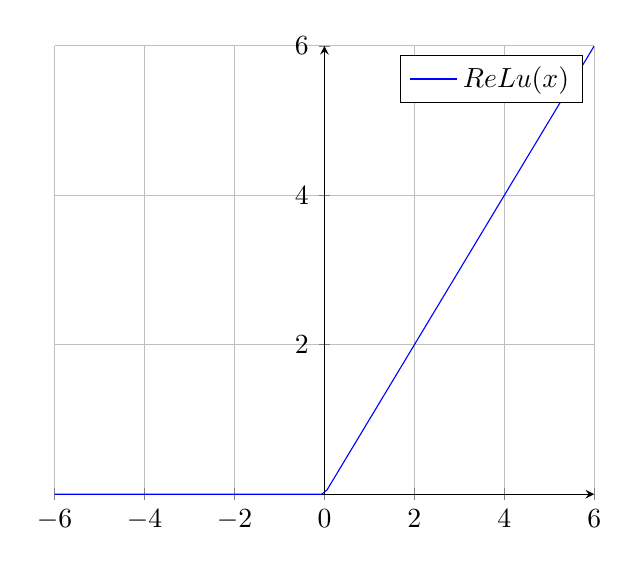
\begin{tikzpicture}[declare function={ReLu(\x)=max(0, x);}]
                        \begin{axis}
                            [
                                grid=major,     
                                axis x line=bottom,
                                ytick={0,2,4,6},
                                axis y line=middle,
                                samples=100,
                                domain=-6:6,
                            ]
                            \addplot[blue,mark=none]   (x,{ReLu(x)});
                            \legend{$ReLu(x)$}
                        \end{axis}
                        \end{tikzpicture}
                    \end{center}
 
                \paragraph*{Leaky ReLu} \mbox{} \\
                \begin{center}
                    \[
                        \text{LeakyReLu}(x) =  \begin{cases}
                                            x < 0 & 0.1 \times x \\
                                            x > 0 & x
                                            \end{cases}
                    \]
                    
                    \vspace{0.2cm}
                    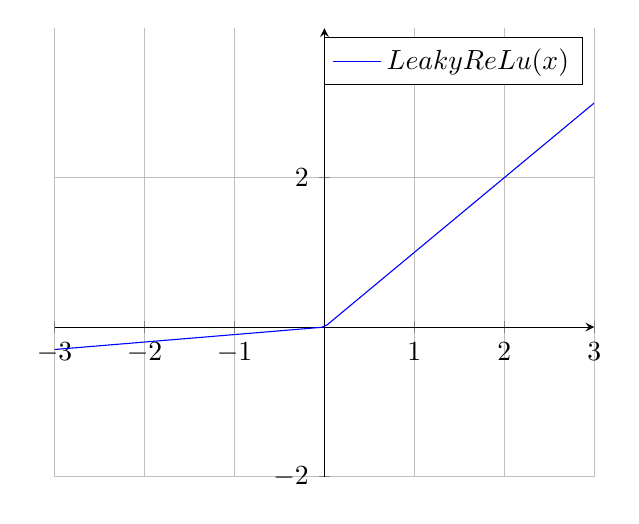
\begin{tikzpicture}[declare function={LeakyReLu(\x)=max(0.1*x, x);}]
                    \begin{axis}
                        [
                            grid=major,     
                            ytick={-2,0,2},
                            axis x line=middle,
                            axis y line=middle,
                            samples=100,
                            domain=-3:3,
                            ymin=-2,
                            ymax=4,
                        ]
                        \addplot[blue,mark=none]   (x,{LeakyReLu(x)});
                        \legend{$LeakyReLu(x)$}
                    \end{axis}
                    \end{tikzpicture}
                \end{center}

                \paragraph*{Sigmoid} \mbox{} \\
                    \begin{center}
                        Sigmoid$(x) = $ \mathLarge{\frac{1}{1 + e^{-x}}} \\
                        \vspace{0.2cm}
                        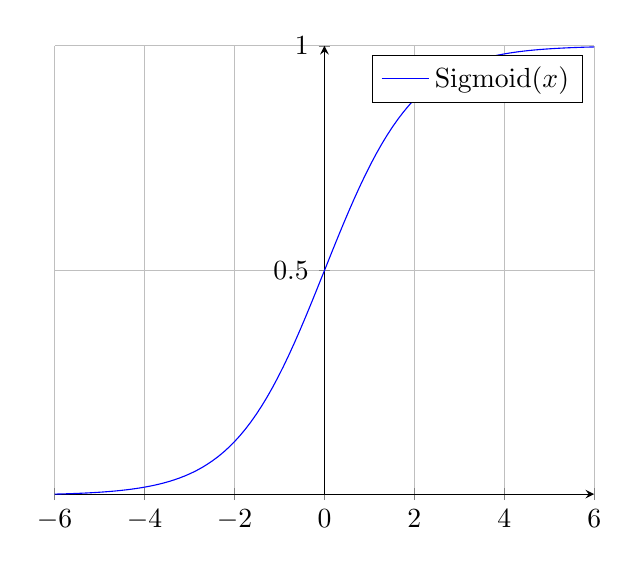
\begin{tikzpicture}[declare function={sigma(\x)=1/(1+exp(-\x));}]
                        \begin{axis}
                            [
                                grid=major,     
                                axis x line=bottom,
                                ytick={-1,-.5,0,.5,1},
                                ymax=1,
                                axis y line=middle,
                                samples=100,
                                domain=-6:6,
                                range=-1:1
                                legend style={at={(1,0.9)}}     
                            ]
                                \addplot[blue,mark=none]   (x,{sigma(x)});
                                \legend{Sigmoid$(x)$}
                        \end{axis}
                        \end{tikzpicture}
                    \end{center}

                \paragraph*{TanH} \mbox{} \\
                    \begin{center}
                        TanH$(x) = $ \mathLarge{\frac{\sinh(x)}{\cosh(x)}} $ = $ \mathLarge{\frac{e^{x} - e^{-x}}{e^{x} + e^{-x}}} \\
                        \vspace{0.4cm}
                        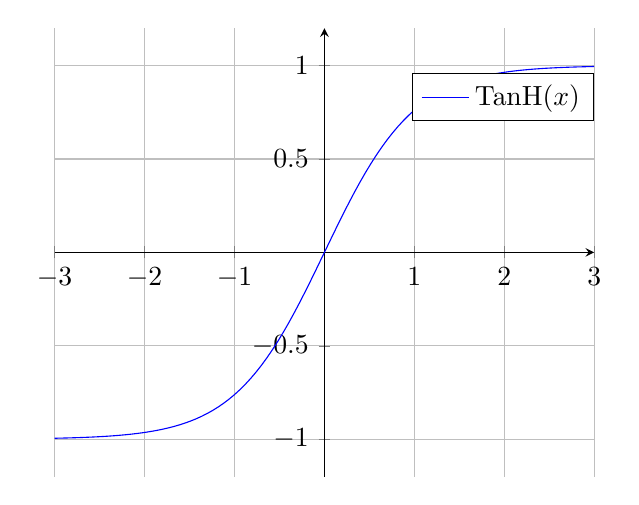
\begin{tikzpicture}[declare function={TanH(\x)=(exp(\x) - exp(-\x))/(exp(\x) + exp(-\x));}]
                        \begin{axis}
                            [
                                grid=major,     
                                axis x line=middle,
                                ytick={-1,-.5,0,.5,1},
                                axis y line=middle,
                                samples=100,
                                domain=-3:3,
                                ymax=1.2,
                                ymin=-1.2,
                                legend style={at={(1,0.9)}}     
                            ]
                                \addplot[blue,mark=none] (x,{TanH(x)});
                                \legend{TanH$(x)$}
                        \end{axis}
                        \end{tikzpicture}
                    \end{center}

                \paragraph{SoftMax} \mbox{} \\
                    SoftMax is slightly different, it is a Generalization of Sigmoid to Multiple Dimensions. It takes in a Vector 
                    \textbf{z} of $K$ Real Numbers, and normalizes it into a probability distribution which Sums to 1. It is commonly used as
                    a logistics function.\\ 

                    \begin{center}
                        \begin{math}
                            \text{SoftMax}(\textbf{z})_{i} = \mathLarge{\frac{e^{z_{i}}}{\sum_{j=1}^{K} e^{z_{j}}}}
                        \end{math} \\
                        \vspace{0.2cm}
                        For $i = 1, \hdots,K$ And \textbf{z} $ = (z_{1},\hdots,z_{K})$ \\
                    \end{center}           
            \subsubsection{Differentiation}
                \paragraph{Differentiation from First Principles}  \mbox{} \\
                    \vspace{0.2cm}
                    Differentiation is the process of finding the Gradient of a Function at a specific point. In the case of a Neural Network,
                    this can be used to measure the sensitivity of the Function Output, in respect to the Input. This derivative is known as said 
                    Functions' Gradient Function. \\
                    \vspace{0.2cm}
                    
                    With a simple straight line graph we can find the gradient as {\Large$\frac{\Delta y}{\Delta x}$, $\Delta$} (Delta) is used to 
                    represent a finite increment. \\
                    \vspace{0.2cm}

                    When find the Derivative of a more Complex Function we can use Two Points. Point $P : (x, f(x))$ and Point $Q : (x + h, f(x + h))$.
                    The variable $h$ tends towards 0, so Points $Q$ will eventually be on top of point $P$. This is called Differentiation from First
                    Principles.
                    \vspace{0.4cm}

                    \begin{eqnarray*}
                        \frac{\Delta y}{\Delta x} &=& \lim_{h\to0} \left(\frac{f(x + h) - f(x)}{(x + h) - x}\right) \\
                        &=& \lim_{h\to0} \left(\frac{f(x + h) - f(x)}{h}\right)
                    \end{eqnarray*}
                    \vspace{0.6cm}

                    Derivatives are more commonly represented as $f'(x)$ or $\frac{dy}{dx}$

                    \vspace{0.4cm}
                \paragraph{Standard Differentiation Rules}  \mbox{} \\
                    \vspace{0.2cm}
                    Instead of manually using Smaller and Smaller Values of $h$ manually, there are standard Differentiation Rules. These are as follows: \\
                    \vspace{0.4cm}

                    \begin{eqnarray*}
                        y = x^{k} &\rightarrow& \frac{dy}{dx} = kx^{k-1} \\
                        y = k &\rightarrow& \frac{dy}{dx} = 0 \\
                        y = e^{kx} &\rightarrow& \frac{dy}{dx} = ke^{kx} \\
                        y = f(x)g(x) &\rightarrow& f(x)g'(x) + f'(x)g(x) \\
                        f(x) = \frac{g(x)}{h(x)} &\rightarrow& f'(x) = \frac{g'(x)h(x) - g(x)h'(x)}{h(x)^{2}} \\
                    \end{eqnarray*}
                    \vspace{0.4cm}

                    These rules are applied to each component of the Function to find the Derivative. 

                \paragraph{Chain Rule}  \mbox{} \\
                    \vspace{0.2cm}
                    The Chain Rule is used to compute the derivative of Nested Functions such as $f(x) = g(h(x))$. The derivative of this Function can be expressed as: \\
                    \vspace{0.4cm}

                    \[f'(x) =  g'(h(x))h'(x)\]

                    \vspace{0.4cm}

                    This can be applied to an infinite number of Functions, where $f(x) = g_{1}(g_{2}(\hdots(g_{n}(x))))$. By this rule we can represent the derivative as
                    a Series of Derivatives Multiplied together:

                    \[
                        \frac{df}{dx} = \frac{df}{df_{1}} \frac{df_{1}}{df_{2}} \frac{df_{2}}{df_{3}} \hdots \frac{df_{n}}{df_{x}}
                    \]

                \paragraph{Partial Derivatives}  \mbox{} \\
                    \vspace{0.2cm}
                    Partial Derivatives are used when the Function in question contains Multiple Variables. They utilise the same rules, except the Variables
                    which aren't being derived get treated as constants. The Derivative of $f(x, y)$ with respect to $x$ is expressed as $f_{x}'(x,y)$ or 
                    {\Large $\frac{\partial f}{\partial x}$}. 
            \subsubsection{Back Propagation}
                \paragraph*{Overview} \mbox{} \\
                    Back Propagation is the algorithm used to adjust Weights and Bias' in a Neural Network. Through using this algorithm you can successfully "train"
                    the Network to recognize certain patterns in data. The Input Data gets propagated through the Network using Forward Propagation, and then the output
                    is passed into the Loss Function. This is being modelled to fulfil \textbf{Objective 5.1.5}.

                \paragraph{The Bellman Equation} \mbox{} \\
                    The Bellman Equation is a method of optimization, and is used for dynamic programming. In the context of Machine Learning we can utilise it
                    to reinforce good behaviour and negate bad behaviour. By writing the relationships between two states in the form of an action, we can optimize this
                    by choosing the best action when given a state. If we let $s_{t}$ be the current state, we can define all the possible actions from that state as
                    $a_{t} \in \Gamma(s_{t})$. Where $\Gamma(s_{t})$ represents all given actions from a state. We can also define the State Transition from $s_{t} \to s_{t+1}$ 
                    as $T(s_{t}, a)$ when action $a$ has been taken. The Reward from this is given as $R(s_{t}, a)$. A Discount Factor $0 < \gamma < 1$ is also defined to assume
                    impatience, compounding the effects of $\gamma$ the further in the future the Reward is. \\
                    \vspace{0.2cm}
                    With these definitions, an infinite-horizon problem is formed: \\

                    \[ V(s_{0}) = \max_{\{a_{t}\}_{t=0}^{\infty}} \sum_{t=0}^{\infty} \gamma^{t} \cdot R(s_{t},a_{t}) \]
                    \vspace{0.2cm}

                    We can form this into another Equation which uses the Principle of Optimality, such that: \\
                    \vspace{0.2cm}

                    \begin{center}
                        \textit{An optimal policy has the property that whatever the initial state and initial decision are, the remaining decisions must constitute an 
                        optimal policy with regard to the state resulting from the first decision.} - Richard E. Bellman
                    \end{center}
                    \vspace{0.2cm}

                    We will consider the first decision separately to all future reward, and then collect the future decisions within the brackets, which the infinite-horizon problem
                    above is equivalent too.

                    \[ \max_{a_{0}} \left\{ R(s_0, a_0) + \gamma \cdot \left[ \max_{\{a_{t}\}_{t=1}^{\infty}} \sum_{t=1}^{\infty} \gamma^{t-1} \cdot R(s_{t},a_{t})\right] \right\} \]
                    \vspace{0.2cm}

                    This at first glance has only made the problem uglier but in fact has made our lives easier. It can be condensed further into a Recursively Defined Function:
                    \vspace{0.2cm}

                    \[ V(s_{0}) = \max_{a_{0}} \{ R(s_{0}, a_{0}) + \gamma \cdot V(x_{1}) \} \] 
                    \centerline{When subjected to: $ x_{1} = T(s_{0}, a_{0})$}
                    \vspace{0.2cm}

                \paragraph{Loss Function} \mbox{} \\
                    The Loss Function of a Network represents how well a Neural Network is performing. The aim of the Back Propagation is to minimize this Functions output. When using
                    a standard Neural Network, and you're training on a labelled data set, you can be certain about the Expected Output. The standard Loss Function is as follows: \\ 
                    \vspace{0.2cm}
                    
                    \begin{eqnarray*}
                        Loss_{i} &=& \frac{1}{2} \cdot (Expected Output_{i} - Actual Output_{i})^{2} \\
                        &=& \frac{1}{2} \cdot (y_{i} - \hat{y}_{i})^{2}
                    \end{eqnarray*}
                    \vspace{0.2cm}

                    This is what's called the Half Square Difference. This Differentiates nicely which is why it is commonly used. \\
                    \vspace{0.2cm}

                    We use the Bellman Equation to calculate the expected value for the loss function.: \\
                    \vspace{0.2cm}

                    \[Q(s_t, a_t) = R(s_t, a_t) + \gamma \cdot \max_{a_{t+1}} Q(s_{t+1}, a_{t+1})\]
                    \[y = \left( R(s_t, a_t) + \gamma \cdot \max_{a_{t+1}} Q(s_{t+1}, a_{t+1}) - Q(s_t, a_t) \right)^2\]

                \paragraph{Gradient Descent} \mbox{} \\ 
                    To minimize the Loss Function, the Weights and Bias' in the Network need to be algorithmically adjusted to converge towards the expected outputs. You can
                    calculate these adjustments by using Partial Derivatives. You can take the Derivative of every Weight and Bias with respect to the Loss Function. The Derivatives
                    of each weight can vary, such as one weight being 0.3 and the other being 3, the Second Weight affects the Loss Function 10$\times$ as much. This process is
                    known as Gradient Descent. \\
                    \vspace{0.2cm}
                    Shown below is a visualization of this process. We can think of Gradient Descent in 3 Dimensions, with the surface representing the Cost of the 
                    Network. To perform Gradient Descent we wish to Minimise the Cost, so when training the Network we make calculated steps towards the 
                    minimum of the surface. In the visualization is shown a dashed yellow line, this represents Gradient Descent in action.

                    \begin{figure}[H]
                        \centering 
                        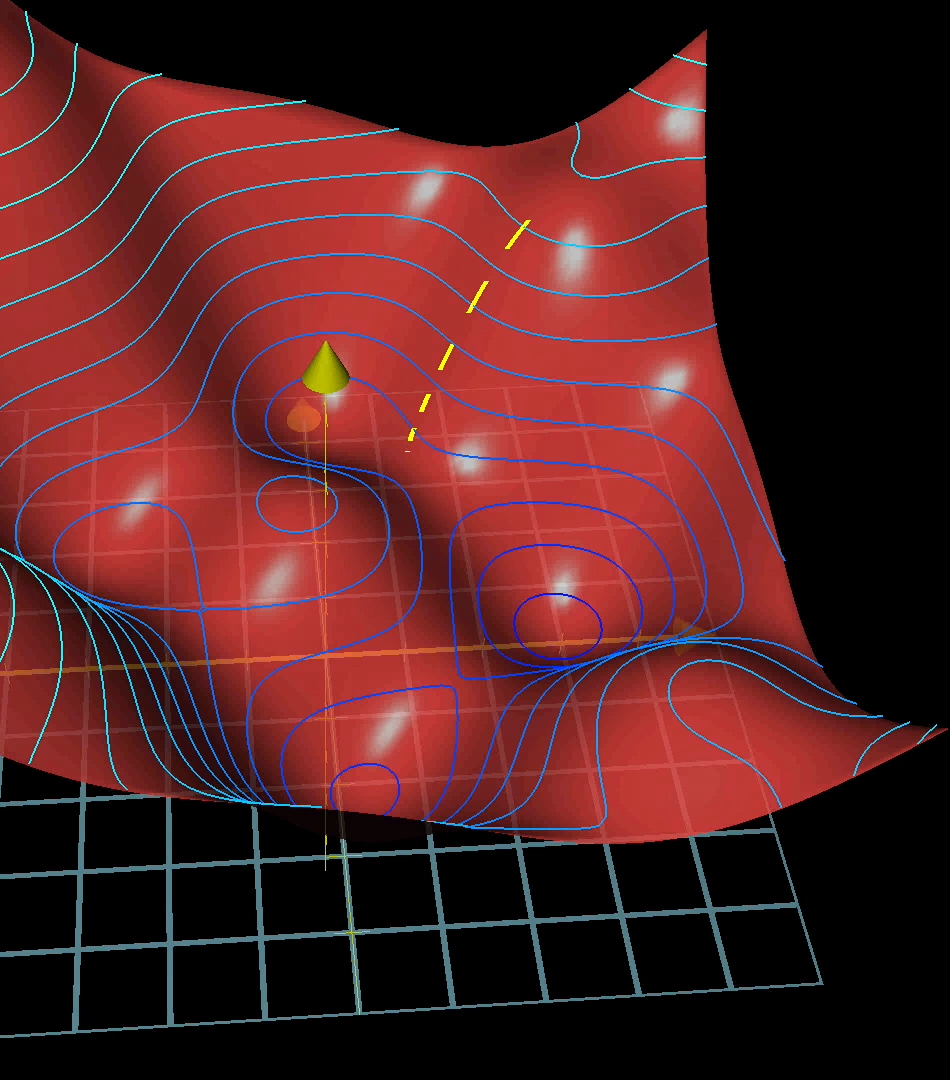
\includegraphics[width=14cm]{Images/ModellingOfProblem/GradientDescent.png}
                        \caption*{Sourced from 3Blue1Brown's Deep Learning Series}
                    \end{figure}

                \paragraph{Differentiating Activation Functions} \mbox{} \\ 
                    As part of Back Propagation we need to derive all the Activation Functions we use within our Layer structure. The Derivatives are shown below. \\
                    \vspace{0.2cm}
                    The ReLu Derivative:
                    \vspace{0.2cm}
                    \[
                        \text{ReLu}(x) =  \begin{cases}
                                            0 & x < 0 \\
                                            x & x > 0
                                            \end{cases} 
                    \]
                    \[
                        \text{Relu'}(x) = \begin{cases}
                                            0 & x < 0 \\
                                            1 & x > 0
                                            \end{cases}
                    \]
                    \vspace{0.2cm}
                    \begin{center}
                        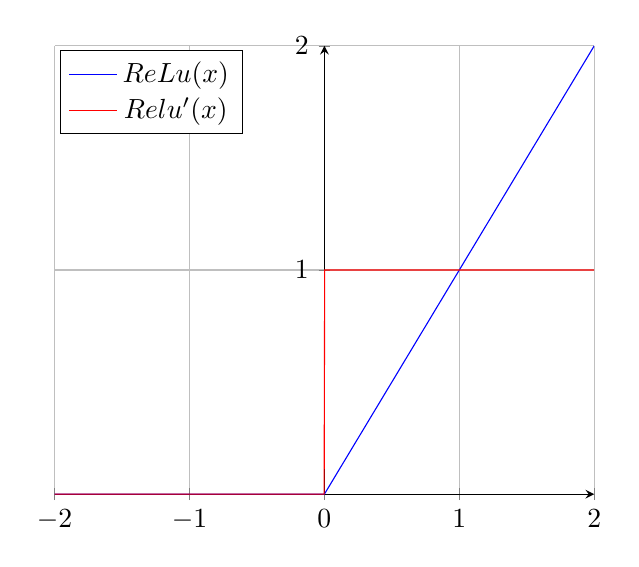
\begin{tikzpicture}[declare function={ReLu(\x)=max(0, x);}]
                        \begin{axis}
                            [
                                grid=major,     
                                axis x line=bottom,
                                ytick={0,1,2,3,4},
                                axis y line=middle,
                                samples=1000,
                                domain=-2:2,
                                legend style={at={(0.01,0.99)},anchor=north west},
                                ymax=2,
                                ymin=0,
                            ]
                            \addplot[blue,mark=none]   (x,{ReLu(x)});
                            \addplot [red,mark=none] {ifthenelse(x>0,1,0)};
                            \legend{$ReLu(x)$, $Relu'(x)$}
                        \end{axis}
                        \end{tikzpicture}
                    \end{center}

                    The Leaky ReLu Derivative:
                    \vspace{0.2cm}
                    \[
                        \text{LeakyReLu}(x) =  \begin{cases}
                                            0.1x & x < 0 \\
                                            x & x > 0
                                            \end{cases} 
                    \]
                    \[
                        \text{LeakyReLu'}(x) = \begin{cases}
                                            0.1 & x < 0 \\
                                            1 & x > 0
                                            \end{cases}
                    \]
                    \vspace{0.2cm}
                    \begin{center}
                        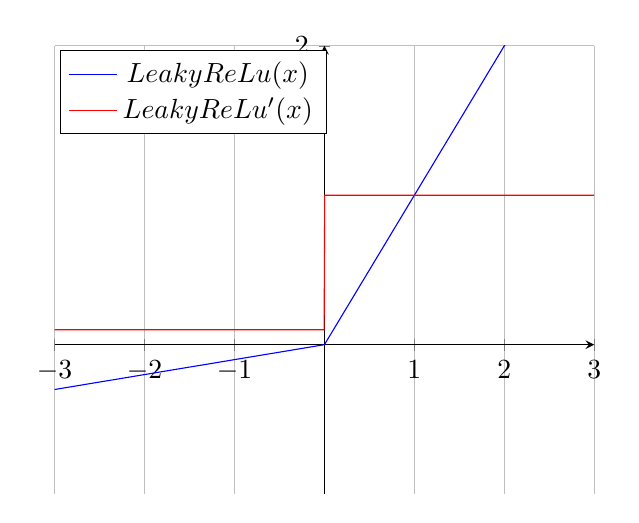
\begin{tikzpicture}[declare function={ReLu(\x)=max(0.1*x, x);}]
                        \begin{axis}
                            [
                                grid=major,     
                                axis y line=middle,
                                samples=1000,
                                legend style={at={(0.01,0.99)},anchor=north west},
                                ytick={-2,0,2},
                                axis x line=middle,
                                domain=-3:3,
                                ymin=-1,
                                ymax=2,
                            ]
                            \addplot[blue,mark=none]   (x,{ReLu(x)});
                            \addplot [red,mark=none] {ifthenelse(x>0,1,0.1)};
                            \legend{$LeakyReLu(x)$, $LeakyReLu'(x)$}
                        \end{axis}
                        \end{tikzpicture}
                    \end{center}

                    The Sigmoid Function Derivative:
                    \vspace{0.2cm}
                    \begin{eqnarray*}
                        \text{Sigmoid}(x) &=& \mathLarge{\frac{1}{1 + e^{-x}}} \\
                                            &=& (1 + e^{-x})^{-1} \\
                        \frac{d\sigma(x)}{dx}&=& -1 \cdot (1 + e^{-x})^{-2} \cdot -e^{-x} \\
                                            &=& \mathLarge{\frac{e^{-x}}{(1 + e^{-x})^{2}}} \\
                                            &=& \mathLarge{\frac{e^{-x}}{1 + e^{-x}} \cdot \frac{1}{1 + e^{-x}}} \\
                                            &=& \mathLarge{\frac{e^{-x} + 1 - 1}{1 + e^{-x}} \cdot \frac{1}{1 + e^{-x}}} \\
                                            &=& \left( \mathLarge{\frac{1 + e^{-x}}{1 + e^{-x}} - \frac{1}{1 + e^{-x}}} \right) \cdot \mathLarge{\frac{1}{1 + e^{-x}}} \\
                                            &=& \text{Sigmoid}(x) \cdot (1 - \text{Sigmoid}(x)) \\
                    \end{eqnarray*}
                    
                    \vspace{0.2cm}
                    \begin{center}
                        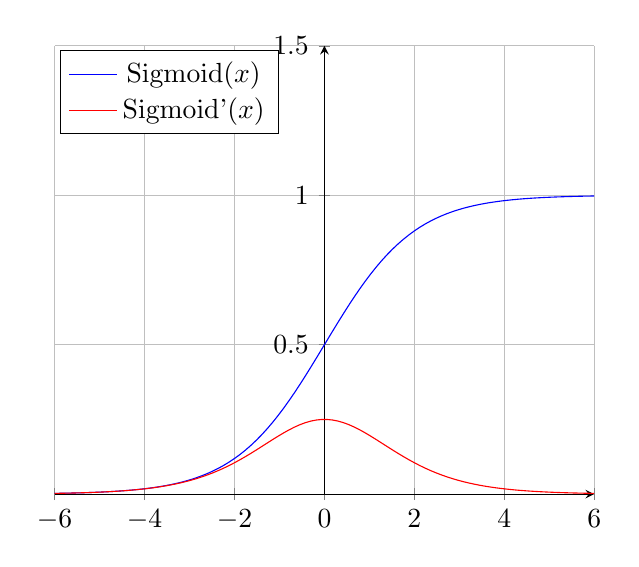
\begin{tikzpicture}[declare function={sigma(\x)=1/(1+exp(-\x));}, declare function={sigmaDer(\x)=sigma(\x)*(1 - sigma(\x));}]
                        \begin{axis}
                            [
                                grid=major,     
                                axis x line=bottom,
                                ytick={-1,-.5,0,.5,1, 1.5},
                                ymax=1.5,
                                ymin=0,
                                axis y line=middle,
                                samples=100,
                                domain=-6:6,
                                legend style={at={(0.01,0.99)},anchor=north west},
                            ]
                                \addplot[blue,mark=none]   (x,{sigma(x)});
                                \addplot[red,mark=none]   (x,{sigmaDer(x)});
                                \legend{Sigmoid$(x)$, Sigmoid'$(x)$}
                        \end{axis}
                        \end{tikzpicture}
                    \end{center}

                    The TanH Derivative:
                    \vspace{0.2cm}
                    \begin{eqnarray*}
                        \text{TanH}(x) &=& \mathLarge{\frac{\sinh(x)}{\cosh(x)}}  \\
                                        &=& \mathLarge{\frac{e^{x} - e^{-x}}{e^{x} + e^{-x}}} \\
                        \text{TanH'}(x)&=& \mathLarge{\frac{(e^{x} + e^{-x})(e^{x} + e^{-x}) - (e^{x} - e^{-x})(e^{x} - e^{-x})}{(e^{x} + e^{-x})^{2}}} \\
                                        &=& \mathLarge{\frac{(e^{x} + e^{-x})^{2}}{(e^{x} + e^{-x})^{2}} - \frac{(e^{x} - e^{-x})^{2}}{(e^{x} + e^{-x})^{2}}} \\
                                        &=& 1 - \text{TanH}^{2}(x) \\
                    \end{eqnarray*}
                    \vspace{0.2cm}

                    \begin{center}
                        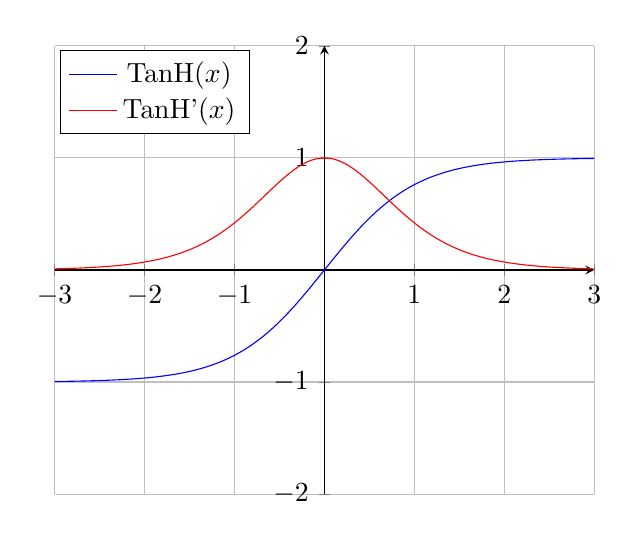
\begin{tikzpicture}[declare function={TanH(\x)=(exp(\x) - exp(-\x))/(exp(\x) + exp(-\x));}, declare function={TanHDer(\x)=1 - TanH(x)^2;}]
                        \begin{axis}
                            [
                                grid=major,     
                                axis x line=middle,
                                ytick={-2,-1,0,1,2},
                                axis y line=middle,
                                samples=100,
                                domain=-3:3,
                                ymax=2,
                                ymin=-2,
                                legend style={at={(0.01,0.99)},anchor=north west}    
                            ]
                                \addplot[blue,mark=none] (x,{TanH(x)});
                                \addplot[red,mark=none] (x,{TanHDer(x)});
                                \legend{TanH$(x)$, TanH'$(x)$}
                        \end{axis}
                        \end{tikzpicture}
                    \end{center}

                \paragraph{Simple Network} \mbox{} \\ 
                    We can apply Back Propagation to this simple Neural Network: \\

                    \begin{figure}[H]
                        \centering 
                        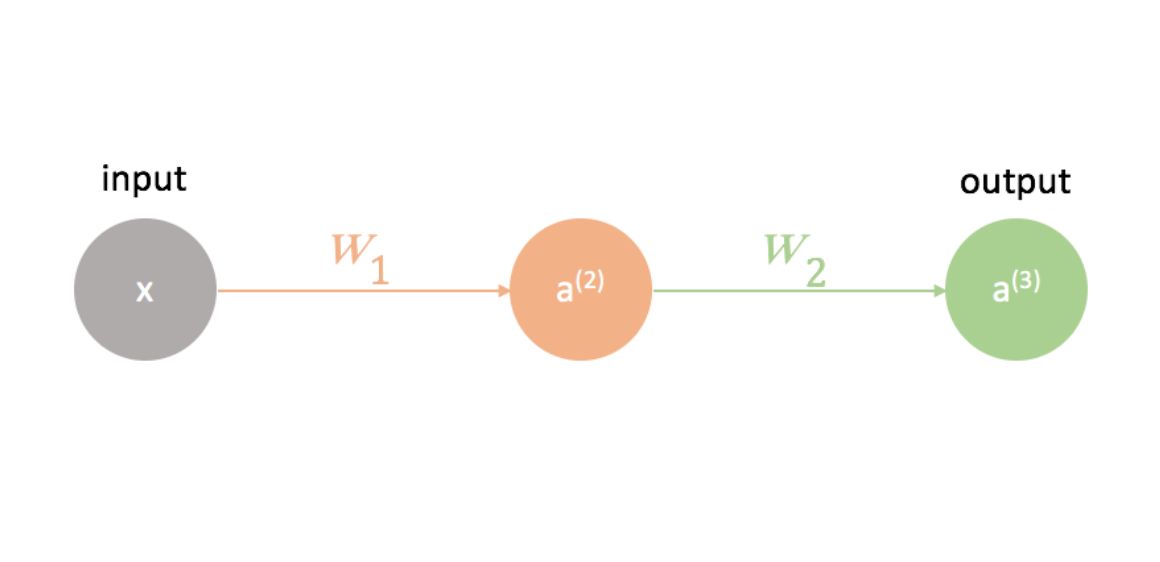
\includegraphics[width=14cm]{Images/ModellingOfProblem/SingleLayerNeuralNetEdited.png}
                        \caption*{Sourced from https://www.jeremyjordan.me/neural-networks-training/}
                    \end{figure}
                    
                    

                    For this Network we need to calculate the derivative of each weight with respect to the cost function. With
                    the use of the chain rule $w_1$ can be expressed as: \\

                    \[\frac{\partial c}{\partial w_{2}} = \frac{\partial c}{\partial a_3} \frac{\partial a_3}{\partial z_3} \frac{\partial z_3}{\partial w_2}\]

                    This means we need to find each derivative in the chain.
                    \vspace{0.2cm}
                    The first derivative is given as $\mathLarge{\frac{\partial c}{\partial a_3}}$. 
                    \begin{eqnarray*}
                        c &=& \frac{1}{2} \cdot (y - a_3)^2 \\
                        \frac{\partial c}{\partial a_3} &=& y - a_3
                    \end{eqnarray*}
                    Next we find $\mathLarge{\frac{\partial a_3}{\partial z_3}}$, here we will use TanH for our activation function.
                    \begin{eqnarray*}
                        a_3 &=& \frac{e^{z_3} - e^{-z_3}}{e^{z_3} + e^{-z_3}} \\
                            &=& \tanh(z_3) \\
                        \frac{\partial a_3}{\partial z_3} &=& 1 - \tanh^{2}(a_3) \\
                    \end{eqnarray*}
                    Next we find the final derivative $\mathLarge{\frac{\partial z_3}{\partial w_2}}$
                    \begin{eqnarray*}
                        z_3 &=& a_2 \cdot w_2 \\
                        \frac{\partial z_3}{\partial w_2} &=& a_2
                    \end{eqnarray*}
                    We then combine this all together to find $\mathLarge{\frac{\partial c}{\partial w_{2}}}$
                    \begin{eqnarray*}
                        \frac{\partial c}{\partial w_{2}} &=& = (y - a_3) \cdot (1 - \tanh^{2}(a_3)) \cdot a_2
                    \end{eqnarray*}

                    \vspace{0.2cm}

                    When calculating the derivatives of $w_1$ it's slightly more complicated, it requires us to \textit{extend}
                    the chain of derivatives.

                    \[\frac{\partial c}{\partial w_1} = \frac{\partial c}{\partial a_3} \frac{\partial a_3}{\partial z_3} \frac{\partial z_3}{\partial a_2} \frac{\partial a_2}{\partial z_2} \frac{\partial z_2}{\partial w_1}\]

                    It is however similar to our original chain, the only new derivative is $\mathLarge{\frac{\partial z_3}{\partial a_2}}$.
                    Which is simply $w_2$, leaving us with the following derivative:
                    \begin{eqnarray*}
                        \frac{\partial c}{\partial w_{1}} &=& (y - a_3) \cdot (1 - \tanh^{2}(a_3)) \cdot w_2 \cdot a_2 \cdot (1 - \tanh^{2}(a_2)) \cdot a_1
                    \end{eqnarray*}

                    We can generalize this into the form below for layers $1,2, \hdots, n$:
                    \begin{eqnarray*}
                        \frac{\partial c}{\partial w_{l}} &=& a_l \cdot \sigma'(z_{l+1}) \cdot \frac{\partial c}{\partial a_{l+1}} \\
                        \frac{\partial c}{\partial a_{l}} &=&
                        \begin{cases}
                            y - \hat{y} & l = n \\
                            w_l \cdot \sigma'(z_{l+1}) \cdot \frac{\partial c}{\partial a_{l+1}} & Else \\
                        \end{cases} 
                    \end{eqnarray*}

                \paragraph{Complex Network} \mbox{} \\ 
                    For a Complex Network, with multiple Neurons per layer, it is quite similar. An example of this is shown below: \\

                    \begin{figure}[H]
                        \centerline{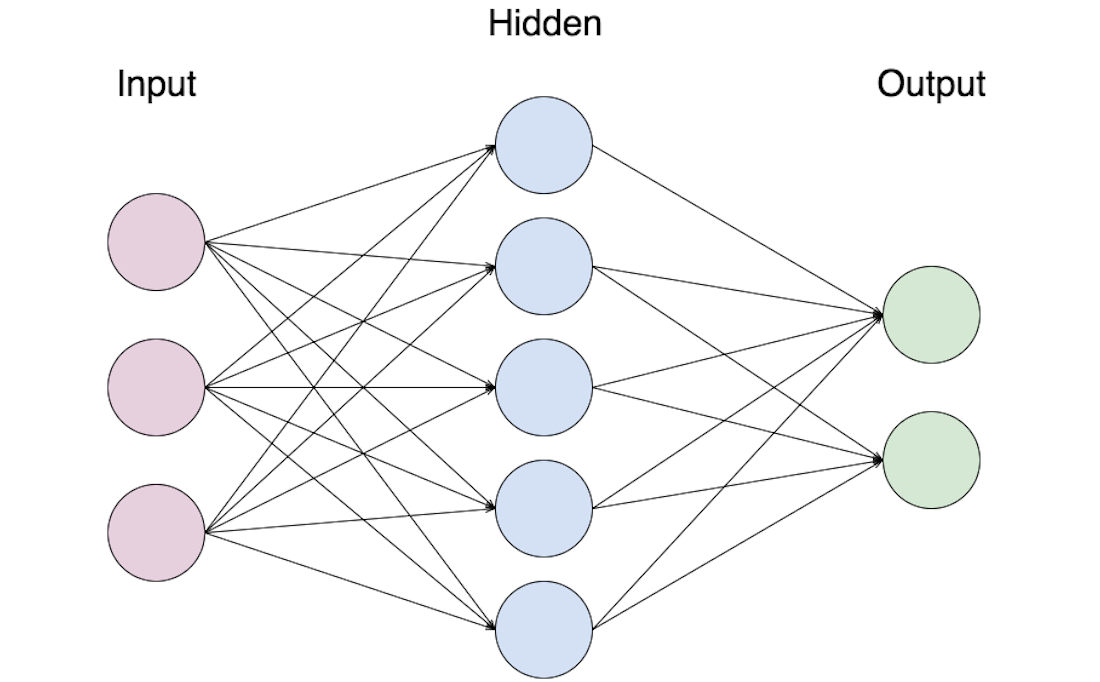
\includegraphics[width=10cm]{Images/InitialResearch/NeuralNetworkExample.png}}
                        \caption*{Sourced from https://webkid.io/blog/neural-networks-in-javascript/}
                    \end{figure}

                    When deriving an Activation value we instead need to consider all weight derivatives connected to the next layer. 
                    We can generalize this into the weight update form for layers $1,2, \hdots, n$:
                    \begin{eqnarray*}
                        \Delta w_{i \to j} &=& -\eta\delta_j z_i \\
                        \delta_i &=& 
                        \begin{cases}
                            \sigma'(z_i) \cdot (y_i - \hat{y}_i) & \text{Node $i$ in Final Layer} \\
                            \sigma'(z_i) \sum_{k\in\text{outs}(i)}  \delta_k w_{i \to k} & Else \\
                        \end{cases}
                    \end{eqnarray*}
                    This should be all that is needed to perform Back Propagation, but we can convert this into it's Matrix form reduce the required
                    operations. Below is defined the needed Matrices which store elements of the Network. \\

                    \begin{align*}
                        Z^{(L)} &=
                        \begin{bmatrix}
                        z^{(L)}_{0} \\
                        z^{(L)}_{1} \\
                        \vdots      \\
                        z^{(L)}_{n} 
                        \end{bmatrix}
                        & W^{(L)} &=
                        \begin{bmatrix}
                        w^{(L-1)}_{0,0} & w^{(L-1)}_{0,1} & \hdots  & w^{(L-1)}_{0,m} \\
                        w^{(L-1)}_{1,0} & w^{(L-1)}_{1,1} & \hdots  & w^{(L-1)}_{1,m} \\
                        \vdots          & \vdots          & \ddots  & \vdots          \\
                        w^{(L-1)}_{n,0} & w^{(L-1)}_{n,1} & \hdots  & w^{(L-1)}_{n,m} \\
                        \end{bmatrix} \\
                        A^{(L)} &=
                        \begin{bmatrix}
                        a^{(L-1)}_{0} \\
                        a^{(L-1)}_{1} \\
                        \vdots      \\
                        a^{(L-1)}_{n} 
                        \end{bmatrix}
                        & B^{(L)} &=
                        \begin{bmatrix}
                        b^{(L)}_{0} \\
                        b^{(L)}_{1} \\
                        \vdots      \\
                        b^{(L)}_{n} 
                        \end{bmatrix}
                    \end{align*}

                    Using these Matrices we then calculate the Weight and Bias derivatives. The Layer N is the final layer, C Networks output with the 
                    Loss Functions derivative applied. This form is shown below: \\

                    \begin{eqnarray*}
                        \delta^{(N)} &=& C \odot \sigma' \cdot Z^{(L)} \\
                        \delta^{(L)} &=& ((W^{(L)})^T \cdot \delta^{(L+1)}) \odot \sigma' \cdot Z^{(L)} \\
                        \beta^{(L)} &=& \delta^{(L)} \\
                        \omega^{(L)} &=& \delta^{(L)} \cdot (A^{(L)})^T \\
                    \end{eqnarray*}
\end{flushleft}